%% abtex2-modelo-artigo.tex, v-1.9.5 laurocesar
%% Copyright 2012-2015 by abnTeX2 group at http://www.abntex.net.br/
%%
%% This work may be distributed and/or modified under the
%% conditions of the LaTeX Project Public License, either version 1.3
%% of this license or (at your option) any later version.
%% The latest version of this license is in
%%   http://www.latex-project.org/lppl.txt
%% and version 1.3 or later is part of all distributions of LaTeX
%% version 2005/12/01 or later.
%%
%% This work has the LPPL maintenance status `maintained'.
%%
%% The Current Maintainer of this work is the abnTeX2 team, led
%% by Lauro César Araujo. Further information are available on
%% http://www.abntex.net.br/
%%
%% This work consists of the files abntex2-modelo-artigo.tex and
%% abntex2-modelo-references.bib
%%

% ------------------------------------------------------------------------
% ------------------------------------------------------------------------
% abnTeX2: Modelo de Artigo Acadêmico em conformidade com
% ABNT NBR 6022:2003: Informação e documentação - Artigo em publicação
% periódica científica impressa - Apresentação
% ------------------------------------------------------------------------
% ------------------------------------------------------------------------

\documentclass[
	% -- opções da classe memoir --
	article,			% indica que é um artigo acadêmico
	11pt,				% tamanho da fonte
	oneside,			% para impressão apenas no verso. Oposto a twoside
	a4paper,			% tamanho do papel.
    % twocolumn,
	% -- opções da classe abntex2 --
	%chapter=TITLE,		% títulos de capítulos convertidos em letras maiúsculas
	%section=TITLE,		% títulos de seções convertidos em letras maiúsculas
	%subsection=TITLE,	% títulos de subseções convertidos em letras maiúsculas
	%subsubsection=TITLE % títulos de subsubseções convertidos em letras maiúsculas
	% -- opções do pacote babel --
	english,			% idioma adicional para hifenização
	brazil,				% o último idioma é o principal do documento
	sumario=tradicional
	]{abntex2}


% ---
% PACOTES
% ---

% ---
% Pacotes fundamentais
% ---
\usepackage{lmodern}			% Usa a fonte Latin Modern
\usepackage[T1]{fontenc}		% Selecao de codigos de fonte.
\usepackage[utf8]{inputenc}		% Codificacao do documento (conversão automática dos acentos)
\usepackage{indentfirst}		% Indenta o primeiro parágrafo de cada seção.
\usepackage{nomencl} 			% Lista de simbolos
\usepackage{color}				% Controle das cores
\usepackage{graphicx}			% Inclusão de gráficos
\usepackage{microtype} 			% para melhorias de justificação
% ---

% ---
% Pacotes adicionais, usados apenas no âmbito do Modelo Canônico do abnteX2
% ---
\usepackage{lipsum}				% para geração de dummy text
% ---

% ---
% Pacotes de citações
% ---
\usepackage[brazilian,hyperpageref]{backref}	 % Paginas com as citações na bibl
\usepackage[alf]{abntex2cite}	% Citações padrão ABNT
% ---

% ---
% Configurações do pacote backref
% Usado sem a opção hyperpageref de backref
\renewcommand{\backrefpagesname}{Citado na(s) página(s):~}
% Texto padrão antes do número das páginas
\renewcommand{\backref}{}
% Define os textos da citação
\renewcommand*{\backrefalt}[4]{
	\ifcase #1 %
		Nenhuma citação no texto.%
	\or
		Citado na página #2.%
	\else
		Citado #1 vezes nas páginas #2.%
	\fi}%
% ---

% ---
% Informações de dados para CAPA e FOLHA DE ROSTO
% ---
\titulo{Sistema de Gerenciamento de manutenção de pontos de iluminação pública
\\ CidadeIluminada}
\autor{Arthur de Paula Bressan \\(IBTA) \and Thais Matias Nogueira \\(IBTA)}
\local{São José dos Campos, Sâo Paulo, Brasil}
\data{2015}
% ---

% ---
% Configurações de aparência do PDF final

% alterando o aspecto da cor azul
\definecolor{blue}{RGB}{41,5,195}

% informações do PDF
\makeatletter
\hypersetup{
     	%pagebackref=true,
		pdftitle={\@title},
		pdfauthor={\@author},
    	pdfsubject={Modelo de artigo científico com abnTeX2},
	    pdfcreator={LaTeX with abnTeX2},
		pdfkeywords={abnt}{latex}{abntex}{abntex2}{artigo científico},
		colorlinks=true,       		% false: boxed links; true: colored links
    	linkcolor=blue,          	% color of internal links
    	citecolor=blue,        		% color of links to bibliography
    	filecolor=magenta,      		% color of file links
		urlcolor=blue,
		bookmarksdepth=4
}
\makeatother
% ---

% ---
% compila o indice
% ---
\makeindex
% ---

% ---
% Altera as margens padrões
% ---
\setlrmarginsandblock{3cm}{3cm}{*}
\setulmarginsandblock{3cm}{3cm}{*}
\checkandfixthelayout
% ---

% ---
% Espaçamentos entre linhas e parágrafos
% ---

% O tamanho do parágrafo é dado por:
\setlength{\parindent}{1.3cm}

% Controle do espaçamento entre um parágrafo e outro:
\setlength{\parskip}{0.2cm}  % tente também \onelineskip

% Espaçamento simples
\SingleSpacing

% ----
% Início do documento
% ----
\begin{document}

% Seleciona o idioma do documento (conforme pacotes do babel)
%\selectlanguage{english}
\selectlanguage{brazil}

% Retira espaço extra obsoleto entre as frases.
\frenchspacing

% ----------------------------------------------------------
% ELEMENTOS PRÉ-TEXTUAIS
% ----------------------------------------------------------

%---
%
% Se desejar escrever o artigo em duas colunas, descomente a linha abaixo
% e a linha com o texto ``FIM DE ARTIGO EM DUAS COLUNAS''.
% \twocolumn[    		% INICIO DE ARTIGO EM DUAS COLUNAS
%
%---
% página de titulo
\maketitle

% resumo em português
\begin{resumoumacoluna}
    Este trabalho apresenta um estudo sobre dispositivos móveis, explicando a implementação de um protótipo de software que auxiliará no recebimento e análise de denuncias relacionados a iluminação pública na cidade de São José dos Campos.
    O aplicativo foi desenvolvido em Android e será responsável por enviar estas denuncias para um ambiente web.
    A aplicação web será responsável por responder às requisições do aplicativo Android e processa-las de modo que a manutenção dos pontos de iluminação pública seja feita de uma maneira mais rápida e menos burocrática.
 \vspace{\onelineskip}

 \noindent
 \textbf{Palavras-chave}: Iluminação pública. Aplicativo Android. Sistema web para manutenção.
\end{resumoumacoluna}

% ]  				% FIM DE ARTIGO EM DUAS COLUNAS
% ---

% ----------------------------------------------------------
% ELEMENTOS TEXTUAIS
% ----------------------------------------------------------
\textual

% ----------------------------------------------------------
% Introdução
% ----------------------------------------------------------
\section*{Introdução}
\addcontentsline{toc}{section}{Introdução}

A Iluminação pública é um instrumento de cidadania, pois é um item essencial à qualidade de vida e a segurança dos centros urbanos, ajudando a preservar e embelezar os patrimônios públicos e a prática de diversas atividade noturnas
no espaço público.

Segundo \cite{aver} a falta de iluminação contribui consideravelmente com o aumento dos índices de criminalidade e a falta de segurança dos cidadãos que por algum motivo tem que transitar no período noturno por pontos sem iluminação, ou com iluminação precária.
Estudos feitos pela organização Campbell Collaboration \cite{newton}, mostraram que a melhoria na iluminação pública em algumas cidades do Reino Unido e EUA, ajudaram a reduzir a criminalidade em até 21\%, e concluiu que esta melhoria promoveu o aumento da vigilância da comunidade, que atuou como elemento inibidor contra a criminalidade local.

Os responsáveis pela instalação e manutenção da iluminação pública dos municípios no Brasil mudaram em dezembro de 2014.
Até então, elas eram feitas pelo estado, normalmente através das concessionárias de energia elétrica.
Agora é a própria prefeitura que tem a responsabilidade por garantir as lâmpadas acessas.
Essa mudança foi ocasionada pela Resolução Normativa 414 \cite{aneel414}, uma determinação constitucional expedida pela ANEEL (Agencia Nacional de Energia Elétrica) que obrigou todos os 5.570 municípios brasileiros a se responsabilizar pela manutenção da infraestrutura da iluminação pública.

A cidade de São José dos Campos/SP conta hoje com cerca de 75.000 pontos de iluminação distribuídos pela cidade.
A média de lâmpadas com defeito é cerca de 900 por mês, de acordo com a Secretaria de Obras da cidade \cite{secretariaobras}.
Um dos maiores problemas a serem enfrentados é o recebimento de chamados para solucionar problemas com os postes defeituosos, já que o canal de reclamações da prefeitura engloba todos os problemas da cidade, causando assim, uma sobrecarga no atendimento.

A Urbanizadora Municipal (URBAM) foi a empresa contratada pela prefeitura de São José dos Campos para realizar a manutenção da iluminação pública do município.
Com a proposta de auxiliar a URBAM no encontro dos pontos com problemas e agilizar as respostas aos chamados abertos pelos munícipes, o trabalho “Cidade Iluminada” apresenta uma solução de um aplicativo para smartphones e uma aplicação Web para a gestão das solicitações de manutenção dos pontos de iluminação pública.

O atual processo de recebimento de chamados, funciona de maneira manual, onde um funcionário deve entrar em um sistema do canal de recebimentos de denuncias, o 156, e coletar manualmente todas as denuncias recebidas no dia, colocar em uma planilha no Excel, e separar por regiões.
Após este passo, a planilha já dividida em regiões, são checados os chamados um a um caso haja duplicidade.
Uma vez que todos os pedidos já estão na planilha e caso não haja duplicidade, uma ordem de serviço é feita e enviada a URBAM para que a manutenção seja feita.
Quando a manutenção é feita, esta ordem de serviço retorna e são retirados da planilha os chamados que foram atendidos.

Evidentemente é um processo muito complexo, e passível a erros, onde por um menor descuido vários detalhes poderão ser perdidos, como denuncias duplicadas que irão gerar o retrabalho quando a ordem de serviço é gerada.
Por isso nós propomos uma solução, onde não será mais necessária a coleta e verificação manual de todas as denuncias.
Todo este trabalho excessivo será reduzido e em poucos cliques toda a análise será feita automaticamente.

Nossa missão é disponibilizar uma ferramenta que irá aperfeiçoar o recebimento dos chamados relacionados aos postes de iluminação e viabilizar a comunicação do cidadão diretamente com a entidade competente através de uma aplicação Android e um ambiente Web onde essas informações serão processadas.
Neste aplicativo, o usuário poderá registrar o problema na rede pública de iluminação, enviar uma foto e a localização do problema e acompanhar o andamento do protocolo aberto por ele.
No ambiente Web, este protocolo será analisado e separado de acordo com a região, bairro, rua e tipo de problemas, também serão analisados se não há duplicidade em algum ponto.
E além disso, o sistema tem como função preparar a ordem de serviço para a manutenção, e fazer o controle dos materiais utilizados.

% ----------------------------------------------------------
% Seção de explicações
% ----------------------------------------------------------
\section{Fundamentação Teórica}

\subsection{Engenharia de Software}

Segundo Pressman, a engenharia de software é definida como: “O estabelecimento e uso de sólidos princípios de engenharia para que se possa obter economicamente um software que seja confiável e que funcione eficientemente em máquinas reais.”\cite{pressman}

O termo engenharia de software foi criado por volta da década de 60, com o objetivo de sanar a crise do software e contornar os problemas oriundos do grande crescimento da demanda de softwares e da complexidade a eles imposta, assim padronizando o desenvolvimento deixando-o mais controlado e sistemático.

Segundo Breitman “o desenvolvimento de sistemas de software é uma atividade complexa que envolve um grande número de recursos, coordenados de modo a atingir um mesmo objetivo”. \cite{breitman}
Por isso esta tarefa exige um planejamento detalhado e documentado por se tratar de um objeto dinâmico que está sempre se adaptando as necessidades dos usuários de acordo com as ferramentas usadas no seu desenvolvimento.
Para Pressman, a engenharia de software tem três fases: definição, desenvolvimento e manutenção \cite{pressman}.

A fase de definição, estabelece as propriedades, características, limitações e funcionalidades do software.
Esta fase é dividida em três etapas, a análise do sistema onde são definidas as funções que o sistema deve apresentar.
O planejamento de projeto, onde  são analisados os riscos, custos e recursos que serão necessários no desenvolvimento.
E por fim a análise dos requisitos, nesta etapa são verificados os requisitos necessários para que atenda as funções do sistema.

A fase de desenvolvimento, é a parte onde os desenvolvedores transformas as especificações em código.
O projeto é analisado, estabelecendo a arquitetura e estrutura dos dados, seguida pela codificação numa linguagem de programação que atenta as necessidades do projeto.

E finalmente a fase de manutenção dedica-se a aprimorar ainda amais o sistema, sendo validado pelo usuário final, que nem sempre está satisfeito.
Algumas mudanças podem ocorrer no projeto final, como correções pontuais que acontecem quando usuário acha um erro, adaptações caso novos atributos precisarem ser adicionados, e por fim o aprimoramento funcional, que acontece a medida que o usuário se acostuma a utilizar o sistema, e poderá sugerir novas funcionalidades.

\subsection{Método de desenvolvimento Agile, Kanban e Scrum}

O Agile foi publicado em 2001 por meio da publicação de um manifesto por Jeff Sutherland, Ken Schwaber et. al. que priorizava a rápida adaptação às novas situações, a colaboração entre si dos times de desenvolvimento, a colaboração dos times de desenvolvimento com os seus clientes e a entrega de softwares que estejam funcionando. \cite{agilemanifesto}
Apesar do Agile não ditar como o desenvolvimento deva ser feito por si só, ele é um conjunto de conceitos para que métodos, como o Kanban e o Scrum, sejam construídos.

O Scrum consiste basicamente em separar atividades de trabalho em sprints, com o objetivo de entregar todas as atividades da forma mais completa possível, trabalhando assim de modo incremental a cada sprint até que o cliente decida que o software esteja com uma qualidade suficiente para ser entregue.
Além disso, seguindo os princípios dos métodos Agile, o Scrum ajuda na colaboração intra-equipe por meio de reuniões stand-up diárias, uma reunião pós-sprint de retrospectiva e uma reunião pré-sprint para planejamento do próximo sprint.
Para facilitar o planejamento, existem somente três “papéis” no Scrum: O Dono do Produto (Product Owner), o Mestre do Scrum (Scrum Master) e a Equipe (Team).

A Equipe consiste nos desenvolvedores que irão efetivamente fazer a implementação do produto baseado nas necessidades do Dono, que é responsável por demonstrar os seus requisitos.
O Mestre do Scrum é responsável por além de transformar os requisitos do Dono em atividades que podem ser divididas entre os membros da Equipe, é responsável principalmente por gerenciar a equipe para que as atividades sejam cumpridas em cada sprint. \cite{scrum}

O Kanban é uma técnica que separa as atividades em estados pré-definidos pela equipe que a utiliza, e é utilizada principalmente para visualizar o progresso de diferentes atividades dentro de um contexto.
Por si só, o Kanban não diz como introduzir novos processos, mas sim como montar os processos existentes, como o Scrum, de forma visual.

\subsection{Resolução Normativa 414}

A Agência Nacional de Energia Elétrica (ANEEL), determinou que a partir de janeiro de 2015, a responsabilidade da manutenção da iluminação pública será do município.
Esta resolução vem de uma determinação da Constituição Federal de 1988 que, em seu artigo 149-A e conforme Emenda Constitucional número 39, de 19 de dezembro de 2002.
A partir desta data limite, o município terá que arcar também com os investimentos para a ampliação e modernização da rede, instalação de medidores de acordo com a concessionária e também a manutenção do cadastro de ativos georreferenciados.

A responsabilidade da manutenção da rede até então era das concessionarias de distribuição de energia elétrica locais.
E segundo uma sondagem da Confederação Nacional dos Municípios (CNM), esse transferência poderá aumentar aproximadamente até 28\% a despensa anual dos municípios.\cite{cdu}

\subsection{Desenvolvimento mobile}

Durante as últimas décadas foi notável o aumento significativo do uso de dispositivos móveis, segundo o grupo Ibope \cite{ibope}, com diversas funções e finalidades específicas, como computadores de bolso, smartphones, telefones celular, consoles portáteis combinado com as mais diversas tecnologias como GPS, navegadores de Internet, WAP, leitores de áudio, vídeo e texto, entre outros, e juntamente com a evolução das tecnologias e o aumento do poder computacional tornou-se possível o desenvolvimento de aplicações independentes do hardware ou software do dispositivo.

Na América Latina não foi diferente, até o ano de 2014 o Brasil possuía certa de 137 milhões de usuário,um pouco mais de 67\% da população, segundo pesquisa conduzida pela eMarketer \cite{emarketer}, que ainda prevê um aumento de mais 4 milhões de usuários até o final de 2015.

Com base nesses dados é irrefutável o crescimento do mercado neste segmento o que propicia muitas oportunidades no desenvolvimento de aplicativos mobile.
É visível a necessidade de encontrar novas soluções para os usuários de smartphones, e integrar novas tenologias a este mercado, pois a necessidade não para de crescer junto com número de usuários.

\subsection{Requisitos do sistema}

Quando pensamos em qualidade de software, o foco está em entender os requisitos estabelecidos para assim evitar, ou minimizar a insatisfação do cliente final.
Segundo Carvalho, Tavares “A demanda por qualidade tem estimulado a comunidade de software para o desenvolvimento de modelos que conduzam a qualidade dos sistemas. Existe uma forte ligação entre requisitos e qualidade.” \cite{tematec}

Em um sistema computacional, os requisitos definem o escopo e os serviços que o sistema deve oferecer, assim como as restrições que são aplicáveis a suas operações.

\section{Tecnologias}

As tecnologias utilizadas foram escolhidas de acordo com o seu nicho específico, tendo em mente que cada uma delas cumpre um papel importante para entregar uma solução de qualidade para o cliente.

\subsection{Python}

Python é uma linguagem de programação multiparadigma (se destacando os paradigmas orientado a objetos e funcional) , interpretada, imperativa e de alto nível; possui tipagem dinâmica e código fonte livre \cite{pythonlicense} e gratuito, que pode ser facilmente encontrado na Internet e podendo ser livremente modificado e redistribuído, e também possui fácil integração com outras plataformas como .NET, Java e C/C++.

A linguagem foi originalmente concebida e implementada pelo holandês Guido Van Rossum no início da década de 1990 \cite{pythonlicense}, e a ideia original era de criar um sucessor para a linguagem ABC.

Uma das grandes vantagens de utilizar o Python é devido à comunidade que surgiu ao redor da linguagem, ocasionando portanto, em um grande número de bibliotecas (cerca de 70,000 pacotes, de acordo com o repositório central Python Package Index)\cite{pypi} tanto open-source como bibliotecas de livre utilização.

O Python foi escolhido para a implementação, junto com o framework web Flask, devido a sua facilidade e velocidade de implementação, além de experiência anteriores com o Python e com o framework Flask.

\subsubsection{Flask}

Flask é um microframework para desenvolvimento web, criado em Python baseado em duas ferramentas Werkzeug, como servidor de aplicação e Jinja2, como o motor de renderização.
O Flask mantém o núcleo simples e, para isso, ele suporta extensões que são capazes de adicionar diversas funcionalidades a aplicação como por exemplo suporte a banco de dados, camadas de cache, geração de formulários, etc.. \cite{flask}

Existem vários outros frameworks de desenvolvimento web para Python, como por exemplo o Django, Pyramid, Tornado, entre outros.
O Flask foi escolhido devido a sua grande capacidade de extensão e por causa de experiências anteriores com o desenvolvimento de aplicativos Web.

\subsubsection{SQLAlchemy e Flask-SQLAlchemy}

O SQLAlchemy é um conjunto de ferramentas para operar com SQL no Python de forma abstrata, englobando assim um ORM e um conjunto de ferramentas para a utilização do SQL no Python de forma natural para os usuários de Python. \cite{sqlalchemy}

Além disso, o SQLAlchemy abstrai os principais bancos de dados, como o MySQL, PostgresSQL, Oracle e até mesmo SQLite.
Isso permite a codificação do acesso ao banco de dados da aplicação sem precisar depender de qual banco específico.

A integração do Flask com o SQLAlchemy se dá por meio da extensão Flask-SQLAlchemy, e ela tem como objetivo principal facilitar a configuração do SQLAlchemy para a sua utilização em aplicativos Flask. \cite{flasksqlalchemy}

O SQLAlchemy e o Flask-SQLAlchemy foram escolhidos devido a sua grande flexibilidade e poder expressivo dentro de sua linguagem, além de sua fácil integração com o Flask.

\subsubsection{Flask-Migrate e alembic}

O alembic é uma ferramenta que trabalha junto com o SQLAlchemy para a geração e execução de migrações de banco de dados.
Isso permite que alterações feitas no código das classes sejam refletidas na estrutura de tabelas no banco de dados de forma semi-automática. \cite{alembic}

O Flask-Migrate é a biblioteca de integração do alembic com o Flask.
Isso expõe ao Flask comandos que facilitam o gerenciamento destas migrações. \cite{flaskmigrate}

O alembic foi escolhido não somente pela sua fácil integração com tanto o SQLAlchemy e o Flask, mas também por ele ser uma ferramenta de gerenciamento de migrações de alta qualidade.

\subsubsection{Flask-Admin}

O Flask-Admin é uma extensão do Flask que auxilia a criação de páginas de gerenciamento do back-end de aplicativos em Flask.
Isso é feito expondo aos programadores utilidades que geram telas administrativas genéricas para que então cada aplicação as customize de acordo com suas necessidades. \cite{flaskadmin}

O Flask-Admin foi escolhido para ser a base das telas do sistema de gerenciamento de ordens de serviço pois grande parte das funcionalidades básicas necessárias para um sistema CRUD já estão maduras no Flask-Admin.

\subsubsection{Flask-Script}

O Flask-Script disponibiliza um conjunto de ferramentas e classes em Python para o gerenciamento da aplicação Flask via linha de comando.

Inicialmente, o Flask-Script disponibiliza comandos para o gerenciamento do servidor de desenvolvimento e disponibiliza estruturas para que cada aplicação possa implementar seus próprios comandos. \cite{flaskscript}
Por exemplo a extensão Flask-Migrate disponibiliza comandos via o Flask-Script para preparar e executar migrações de banco de dados.

O Flask-Script foi escolhido para realizar a integração pois ela atende satisfatoriamente à demanda de auxílio no gerenciamento da aplicação.

\subsubsection{xhtml2pdf}

O xhtml2pdf é uma biblioteca que tem como objetivo transformar páginas HTML preparadas para o formato PDF.\cite{xhtml2pdf}

A biblioteca foi utilizada para gerar as tabelas das ordens de serviço para compartilhar com a URBAM os endereços dos postes de cada ordem de serviço gerada.

Essa biblioteca foi utilizada pois ela era a mais conveniente de ser utilizada dado o fato que o Flask contém um renderizador de templates HTML.

\subsubsection{fabric e fabtools}

O fabric é uma utilidade que tem como objetivo executar comandos de gerenciamento de servidores via SSH.
A grande vantagem de sua utilização é automatizar tarefas de lançamento da aplicação ou até mesmo a preparação de ambientes de produção.\cite{fabric}

O fabtools é uma biblioteca que expande o fabric para que a escrita de scripts fabric seja ainda mais fácil.
Para isso, o fabtools expõe comandos para as ferramentas mais utilizadas, como comandos do sistema de arquivos, gerenciamento de pacotes de instalações, git, banco de dados, etc.. \cite{fabtools}

O fabric e fabtools foram escolhidos para serem utilizados devido experiências positivas anteriores de gerenciamento de servidores.

\subsubsection{unicodecsv}

O módulo csv do Python é disponibilizado na biblioteca padrão do Python para a leitura e escrita de arquivos separados por vírgula.
Porém, devido às dificuldades do Python 2.7 para a leitura e uso de textos com codificação em Unicode, surgiram várias bibliotecas que vieram para suplantar os módulos da biblioteca padrão.

Uma dessas bibliotecas é justamente o unicodecsv, que simplesmente faz o tratamento de textos em Unicode para que não ocorra erros na leitura e escrita desses arquivos com a codificação Unicode. \cite{unicodecsv}

Ela foi escolhida pois, além de atender perfeitamente essa demanda, ela tem uma grande facilidade no seu uso, pois a sua interface e idêntica ao módulo csv padrão do Python

\subsubsection{Flask-Security}

O Flask-Security é a integração de uma série de bibliotecas do Flask relacionadas ao controle de acesso de usuários com o objetivo de facilitar a implementação desse tipo de sistema. \cite{flasksecurity}

Apesar de sua baixa flexibilidade, o Flask-Security foi escolhido para ser usado no controle de acesso pois ele atendia plenamente as necessidades do projeto na questão de gerenciamento de usuários e controle de acesso.

\subsection{Java}

A linguagem de programação Java foi lançada em 1995, e, desde o início de seu desenvolvimento em 1993 ela foi especificada para ser “independente de plataformas, porém segura o suficiente para atravessar redes e poderosa o suficiente para substituir código nativo”. \cite{java}

O Java teve as mais diversas aplicações, sendo usado para applets para a Web, para programas desktop, para serviços em servidores, para aplicações Web e até rodando em sistemas embarcados.
Essa última aplicação provavelmente possibilitando a implementação do sistema operacional para smartphones Android.

O Java foi utilizado para a implantação do aplicativo Android do Cidade Iluminada pois é a linguagem que o sistema operacional Android usa nativamente para as aplicações, tornando assim o desenvolvimento do aplicativos de acordo com os padrões de desenvolvimento Android.

\subsubsection{Android}

O sistema operacional Android foi lançado pela Google no ano de 2007, e no ano de 2008 foi lançado uma API para os desenvolvedores.
Desde o seu lançamento, este sistema operacional obteve grande popularidade em seu uso, chegando a ter mais de 89\% do mercado brasileiro no primeiro trimestre de 2015, segundo o site Kantar Worldpanel ComTech. \cite{comtech}
A Google provê uma API de fácil manipulação, com código fonte aberto baseada em Java para incentivar e simplificar o desenvolvimento de aplicações, o que tem sido uma boa estratégia já que o número de aplicativos disponíveis no Android Market chegou a 1.6 milhões no último semestre de 2015.

O sucesso do Android no mercado brasileiro, que segundo a pesquisa do site The Statistics Portal, o market share do sistema operacional chegou a mais de 77\% no primeiro semestre de 2015 \cite{statista}, e a facilidade de desenvolvimento foram os principais motivos da escolha do uso deste para o desenvolvimento do aplicativo Cidade Iluminada.

\subsubsection{GSON}

GSON é uma biblioteca do Google para a serialização e deserialização de objetos Java arbitrários.
O objetivo desta biblioteca, além de prover essas conversões, é trabalhar com objetos que o programador não necessariamente tem o código-fonte disponível, mantendo uma interface simples para quando for precisar converter de e para JSON. \cite{gson}

A biblioteca foi utilizada pois ela atende a necessidade principal de tratar JSON mas ainda sendo relativamente fácil de utilizar e configurar as classes que precisam dessa conversão.

\subsubsection{Joda-Time}

A biblioteca Joda-Time tem como objetivo prover facilidades para o programador Java manipular objetos de data e tempo, tendo em vista que a biblioteca padrão do Java deixa a desejar no aspecto de facilidade de uso.

Ela foi utilizada para a geração de timestamps em UTC para marcar o envio das requisições do aplicativo e para gerar os nomes de arquivos das fotos tiradas pelo aplicativo.
A biblioteca Joda-Time foi escolhida para substituir a biblioteca padrão do Java nas suas proximas versões.\cite{jodatime}

\subsubsection{Retrofit}

A biblioteca Retrofit tem como objetivo disponibilizar ferramentas para que se possa definir APIs REST como interfaces Java para serem então usadas no código da aplicação sem maiores dificuldades.
Além disso, ela disponibiliza modos de fazer requisições síncronas ou assíncronas, dependendo das necessidades de cada aplicação.\cite{retrofit}

A biblioteca Retrofit foi utilizada devido a sua facilidade de utilização e adaptação à API já definida do trabalho.

\subsubsection{Sugar}

Sugar é uma biblioteca que tem como objetivo de ser uma ORM especificamente para aplicações Android, tendo uma interface por objetos e classes com o banco de dados SQLite do dispositivo.
Além disso, ela tem a pretensão de ser simples de usar e simples de configurar, além de possuir suporte à migraçoes de banco automáticas.\cite{sugar}

O Sugar foi escolhido justamente devido a sua simplicidade tanto na configuração quanto no seu uso dentro do codigo.

\subsection{JavaScript}

JavaScript é uma linguagem dinâmica, funcional e orientada a objetos, suas aplicações são distribuídas somente em forma de código fonte, e é executada em todos os navegadores modernos com poucas ou nenhuma diferença de plataforma.
Isso é especialmente importante nos dias atuais pois até mesmo smartphones têm o seu próprio navegador, abrindo então uma nova plataforma inteira de aplicações.

Feita em 1994 para a Netscape por Brendan Eich, é a linguagem utilizada para dar interações mais ricas à páginas web.
Apesar de sua idade, a linguagem foi passando por várias alterações que a deixam muito mais poderosa e mais em linha com as necessidades atuais de desenvolvimento para a Web moderna.

O JavaScript foi escolhido para a implementação de páginas Web dinâmicas no projeto principalmente pelo fator de ele ser suportado pelos principais navegadores existentes no mercado, como o Mozilla Firefox, o Google Chrome e o Internet Explorer, sendo os dois primeiros softwares livres para a utilização em ambientes pessoais ou corporativos.

\subsubsection{JSON}

JSON (JavaScript Object Notation) é um formato para guardar e transmitir dados em formato de texto.
O JSON foi descoberto e formalizado por Douglas Crockford em 2001. \cite{json}
Desde então vem ganhando popularidade como um formato de troca de dados entre aplicações web.
Existem bibliotecas para a leitura do formato JSON para a maioria das linguagens de programação, além do suporte praticamente nativo no JavaScript e Python.

O JSON foi escolhido como método de troca de dados pois ele tem suporte praticamente nativo em JavaScript e Python, além de ser mais eficiente em termos de quantidade de bytes enviados do que XML para envio de dados mais simples.

\subsubsection{AngularJS}

AngularJS é um framework do tipo MVC (Model-View-Controller) JavaScript que tem como objetivo facilitar o desenvolvimento web, estendendo e adaptando o HTML para melhorar a experiência de desenvolvimento de páginas Web altamente dinâmicas.
Esta framework foi criada em 2009 por Miško Hevery e Adam Abrons, e é open-source. \cite{angularjs}

O framework foi utilizado na criação da página de controle dos protocolos vindos da aplicação Android, sendo parte fundamental da implementação do módulo de tempo real desta página.

O AngularJS foi escolhido devido a sua grande capacidade de facilitar o desenvolvimento e manutenção de páginas Web altamente interativos.

\subsubsection{JQuery}

JQuery é uma biblioteca JavaScript que tem como objetivo principal facilitar a seleção e manipulação de documentos HTML e o controle de eventos nas páginas.
Isso possibilita a criação de páginas interativas em JavaScript com muito menos dificuldades.
Além disso, o JQuery disponibiliza uma API única para todos os navegadores principais. \cite{jquery}

O JQuery foi utilizado em várias das páginas da parte de gerenciamento de protocolos e serviços, pois ela se tornou uma peça fundamental para o desenvolvimento Web moderno.
Das páginas utilizadas, destaca-se a página de criação de Ordens de Serviço, onde a parte de seleção de postes foi implementada em JQuery.

\subsection{Representational State Transfer (REST)}

O REST é um estilo de arquitetura para aplicações Web proposta por Roy Thomas Fielding em sua dissertação de PhD. \cite{fielding}
Esta tese tinha como objetivo de, além de propor esse tipo de arquitetura, avaliar se serviços disponíveis na Web até então seguiam os quesitos seguintes:

\begin{itemize}
\item \textbf{Cliente-Servidor:} A aplicação teria que manter independentemente suas implementação de clientes (interface gráfica, por exemplo) da implementação dos serviços oferecidos por ela (banco de dados, por exemplo)

\item \textbf{Sem estado:} Isso significa que, a cada requisição enviada para o servidor, esta teria que incluir todos os dados para que a própria seja entendida, sem que o servidor precise depender de informações que por ventura ele possa ter armazenado anteriormente.

\item \textbf{Cacheável:} Cada resposta a uma requisição tem que deixar explícito se é permitido guardar a resposta em um cache no cliente.
A ideia é que, se o cliente precisar refazer uma requisição equivalente, esta requisição deveria utilizar o cache ao invés de ser re-enviada para o servidor.

\item \textbf{Interface uniforme:} De acordo com Fielding em sua dissertação, é a característica fundamental que aplicações REST têm de implementar.
Ela consiste em padronizar todos os componentes para que as implementações de clientes e serviços sejam simplificados.

\item \textbf{Sistema em camadas:} Cada componente deve não conhecer ou depender de componentes de que este componente não precise interagir.
A principal vantagem, de acordo com Fielding, é que o sistema em camadas pode ser usado para encapsular clientes e serviços legados.

\item \textbf{“Code-on-demand”:} A aplicação REST teria que oferecer um conjunto de recursos que viriam como código a ser executado no cliente.
Este código seria como uma interface mínima da aplicação para o cliente consumir.
A principal vantagem de implementar o Code-on-demand seria que a parte básica da API não precisaria ser reimplementada pelo cliente.
É o único quesito opcional para que uma interface fosse considerada como REST.
\end{itemize}

\section{Desenvolvimento}

O desenvolvimento do trabalho pode ser separado em duas fases ou períodos distintos, sendo estes o desenvolvimento do aplicativo para smartphones Android e o sistema de gerenciamento dos protocolos deste, e o desenvolvimento do sistema de gerenciamento de pontos de iluminação e de seus serviços e chamados.

\subsection{Aplicativo Android e seu sistema de gerenciamento}

Para o desenvolvimento do aplicativo para smartphones Android e seu sistema de gerenciamento, foram aplicadas os métodos Agile de desenvolvimento Scrum e Kanban.

As atividades a serem cumpridas foram determinadas no início do projeto, e foram divididas em três categorias, e priorizadas dependendo da importância de cada atividade para o cumprimento do projeto.

Em relação à execução das atividades, elas foram divididas em 5 “sprints”, que foi um período de 14 dias em que as atividades selecionadas para fazer parte do sprint teriam que ser cumpridas.
Para determinar quais atividades entrariam em cada sprint, foi usado primeiramente o critério da prioridade de cada atividade, e secundariamente, o tempo estimado para o término da atividade.

\subsubsection{Backlog de atividades}

O backlog de atividades é o repositório inicial das atividades, e onde cada atividade foi posta em uma das três categorias de desenvolvimento, App, Webservice e Site Secretaria.
Além disso, cada atividade recebeu uma pontuação de 1 a 15, que determinava a prioridade daquela atividade. 1 é a atividade mais prioritária.

\begin{table}[htbp]
    \caption{Tabela de definição das atividades.}
    \label{tabela-atividades}
    \begin{center}
        \begin{tabular}{|p{5cm}|p{4cm}|p{5cm}|}
            \hline
            8 - Tela Principal & 7 - Incluir protocolos & 1 - Criar Banco de Dados \\
            9 - Incluir protocolos anônimos & 13 - Consultar protocolos & 2 - Página inicial \\
            10 - Cadastro de usuário & 14 - Listar protocolos & 3 - Cadastro de usuário \\
            11 - Incluir protocolos cadastrados & & 4 - Controle de acesso \\
            12 - Gravar off-line protocolos para envio posterior & & 5 - Visualizar protocolos \\
            15 - Listar protocolos & & 6 - Mudar status protocolos \\
            \hline
        \end{tabular}
    \end{center}
\end{table}

\subsubsection{Definição dos Sprints}

Um sprint é um período previamente acordado pelo time Agile onde o sistema é de fato implementado.
Este período pode variar de acordo com cada equipe, mesmo em equipes dentro da mesma organização ou empresa.

Para o desenvolvimento do sistema de gerenciamento dos protocolos e do aplicativo Android, cada sprint teve duração de 14 dias, onde foram escolhidos várias atividades de acordo com os critérios da sua prioridade de implementação e sua facilidade de implementação dada a situação que o projeto se encontrava.

\begin{description}
\item[Sprint I:]
O primeiro sprint foi feito a modelagem e a implementação do banco de dados, assim como o layout e a wireframe do ambiente web.

\item[Sprint II:]
Nesta segunda etapa foi feita a criação do layout e padronização da interface do ambiente web.
Também foram implementados os serviços de criação e inclusão dos protocolos.

\item[Sprint III:]
Implementação das telas do aplicativo Android, e do fluxo principal de telas, também como a funcionalidade de ativar a câmera do aparelho, também foi implementado uma funcionalidade que busca automaticamente a localização do aparelho que está enviando o reporte.

\item[Sprint IV:]
Este sprint foi focado na implementação das funcionalidades do aplicativo como o cadastro do usuário, tela de configurações e status dos protocolos enviados

\item[Sprint V:]
No último sprint foram acertado os últimos detalhes do aplicativo, como gravação dos protocolos off-line para envio posterior, busca do status do protocolo e foi finalizado o design da aplicação.
\end{description}

\subsubsection{Apresentação para a Secretaria de Obras}

Após a finalização da primeira versão do aplicativo e do ambiente web do projeto “Cidade Iluminada”, fomos convidados a apresentar nossa solução para o Secretário de Obras de São José dos Campos, o senhor Rene Mina Vernice e sua equipe, na data de 14 de Maio de 2015.

Inicialmente, a ideia do aplicativo não foi bem aceita, pois foi alegado que isso geraria ainda mais trabalho para os funcionários responsáveis por recolher as denuncias relacionadas a iluminação pública.
Apesar disso, o conceito do ambiente web para gerenciamento foi bem recebido, pois eles enfrentam muitas dificuldades administrando os chamados já existente.

\subsubsection{Fluxo de utilização do aplicativo}

A seguir será descrito o fluxo principal de utilização do aplicativo Android para os munícipes.

Para enviar uma solicitação pelo aplicativo, o usuário deve iniciar a aplicação (Figura \ref{android-tela-inicial}), e clicar em Abrir Chamado, na próxima tela (Figura \ref{android-tela-nova-chamada}) serão solicitados uma alguns dados sobre a chamada.

\begin{figure}[!htbp]
 \centering
  \begin{minipage}{0.4\textwidth}
    \centering
    \caption{\label{android-tela-inicial}Tela inicial}
    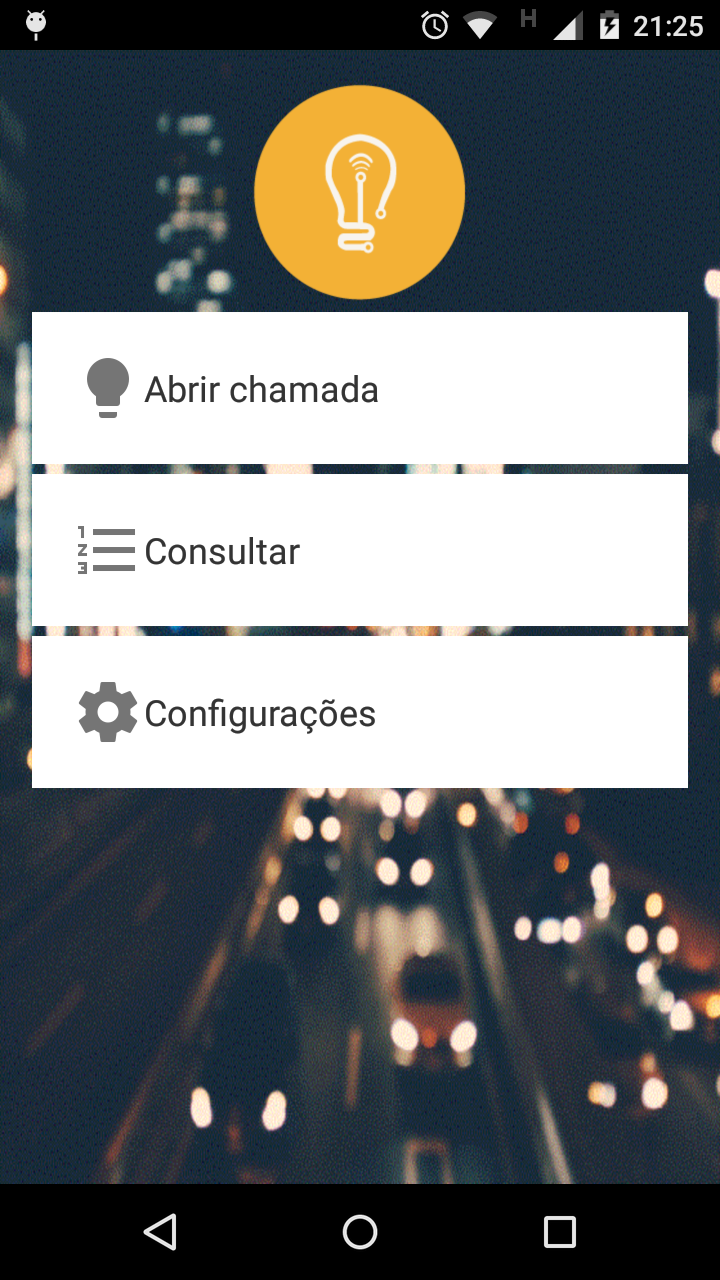
\includegraphics[scale=0.1]{android/1.png}
    \legend{Fonte: Produzido pelos autores}
  \end{minipage}
  \hfill
  \begin{minipage}{0.4\textwidth}
    \centering
    \caption{\label{android-tela-nova-chamada}Tela de nova chamada}
    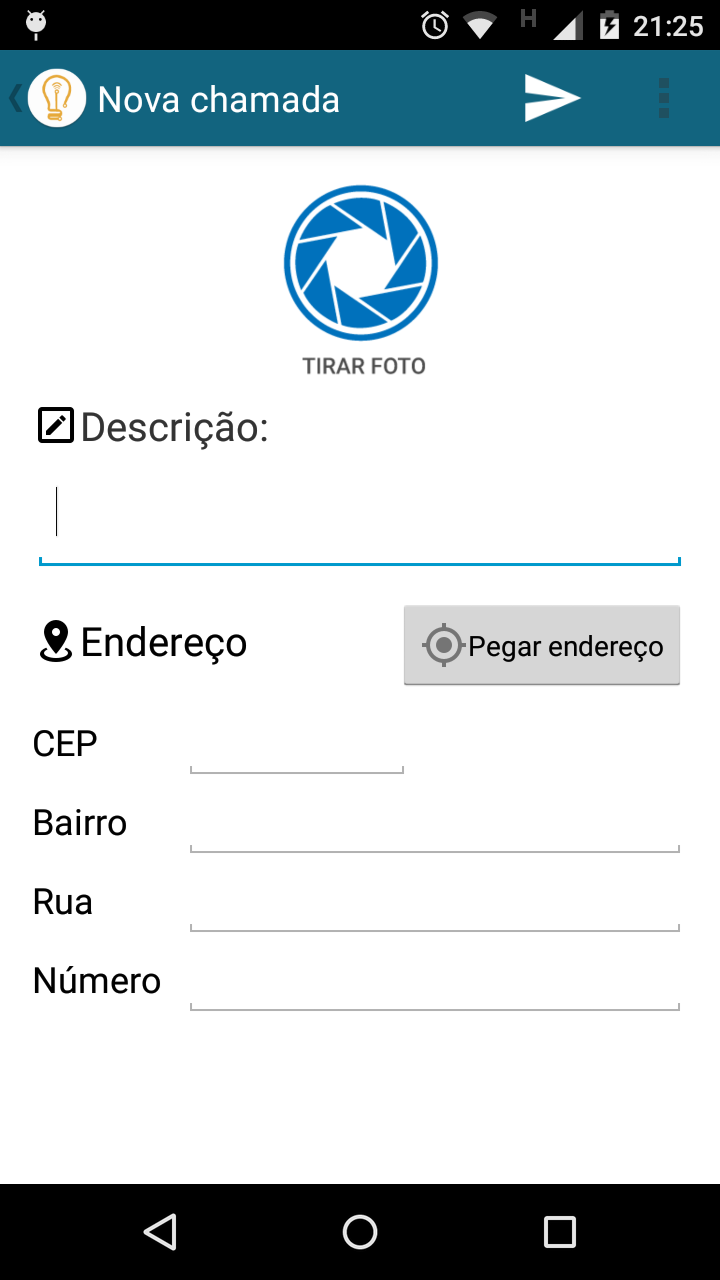
\includegraphics[scale=0.1]{android/2.png}
    \legend{Fonte: Produzido pelos autores}
  \end{minipage}
\end{figure}

Primeiramente, deve-se tirar uma foto do poste defeituoso (Figura \ref{android-tela-nova-chamada-foto-poste}) e em seguida selecionar a localização na tela de seleção de endereço via GPS (Figura \ref{android-tela-gps}), assim o endereço é preenchido automaticamente (Figura \ref{android-tela-nova-chamada-endereco}).

\begin{figure}[!htbp]
 \centering
  \begin{minipage}{0.4\textwidth}
    \centering
    \caption{\label{android-tela-nova-chamada-foto-poste}Tela de chamada com a foto do poste}
    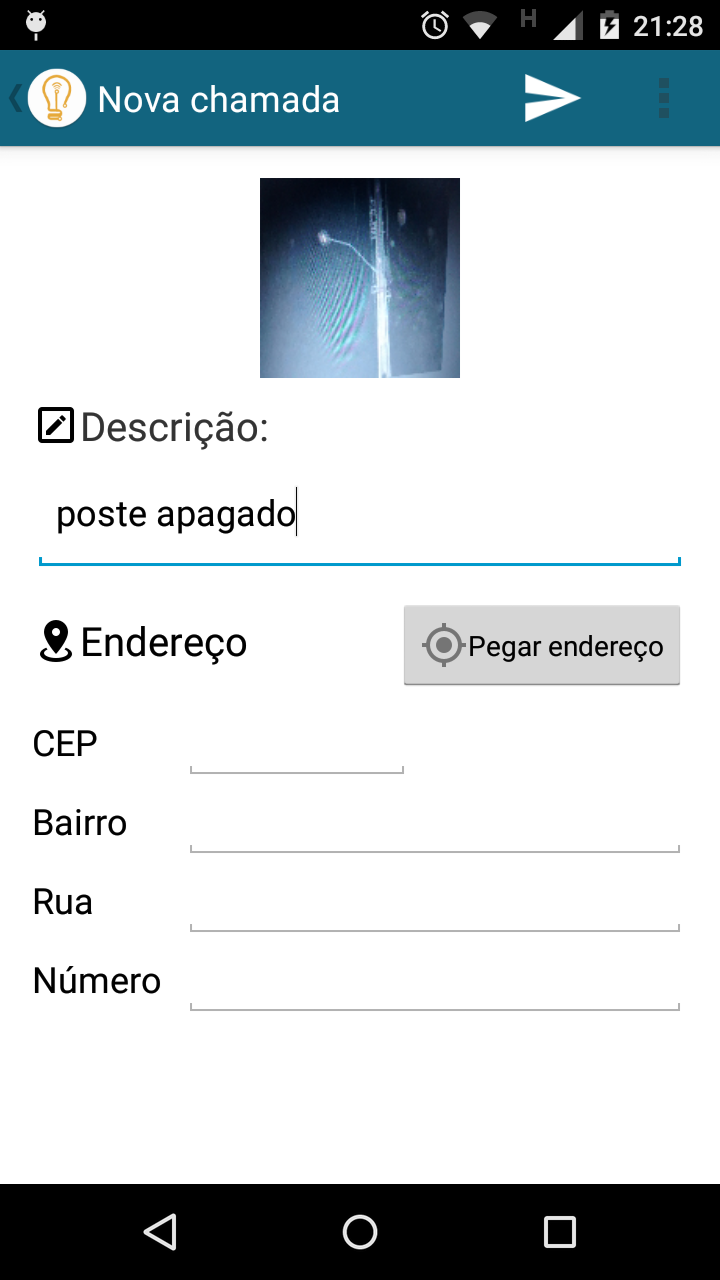
\includegraphics[scale=0.1]{android/3.png}
    \legend{Fonte: Produzido pelos autores}
  \end{minipage}
  \hfill
  \begin{minipage}{0.4\textwidth}
    \centering
    \caption{\label{android-tela-gps}Tela de seleção de endereço via GPS}
    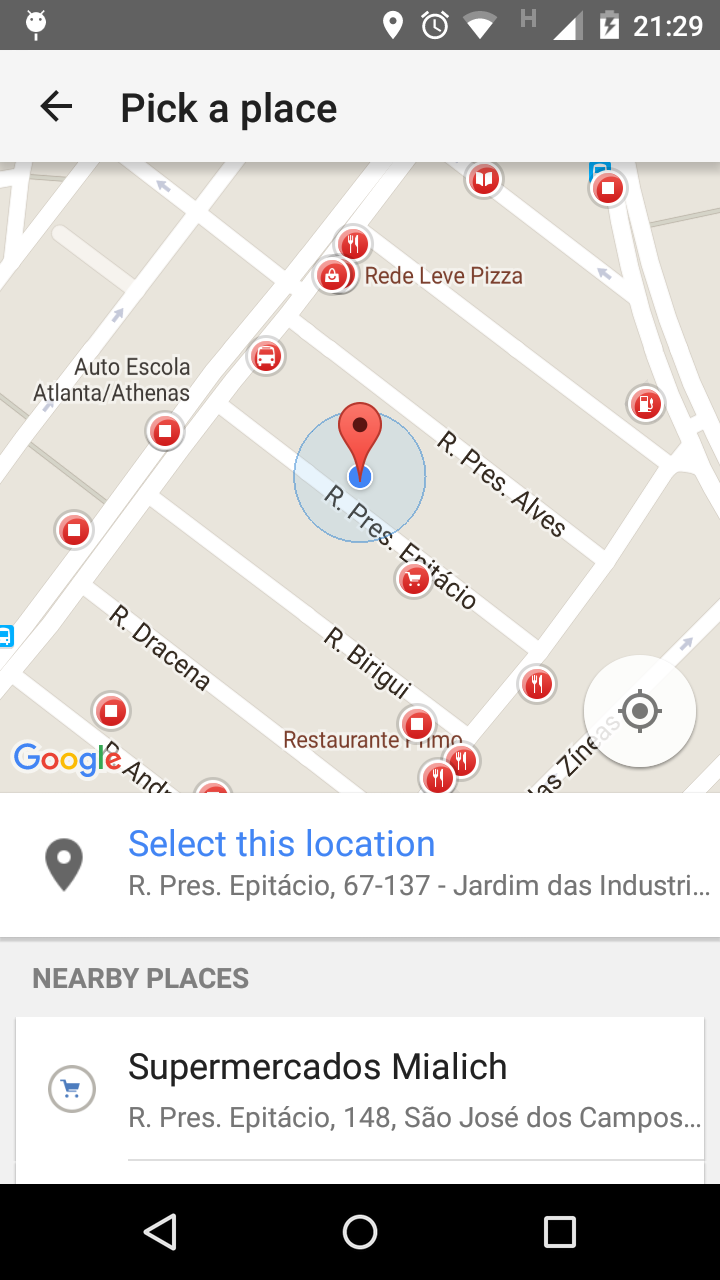
\includegraphics[scale=0.1]{android/4.png}
    \legend{Fonte: Produzido pelos autores}
  \end{minipage}
\end{figure}


Após a coleta dos dados, o usuário deve clicar em enviar protocolo e logo a seguir, o aplicativo irá iniciar a transferência dos dados para o servidor (Figura \ref{android-tela-enviando}).

\clearpage

\begin{figure}[!htbp]
 \centering
  \begin{minipage}{0.4\textwidth}
    \centering
    \caption{\label{android-tela-nova-chamada-endereco}Tela de chamada com o endereço preenchido automaticamente}
    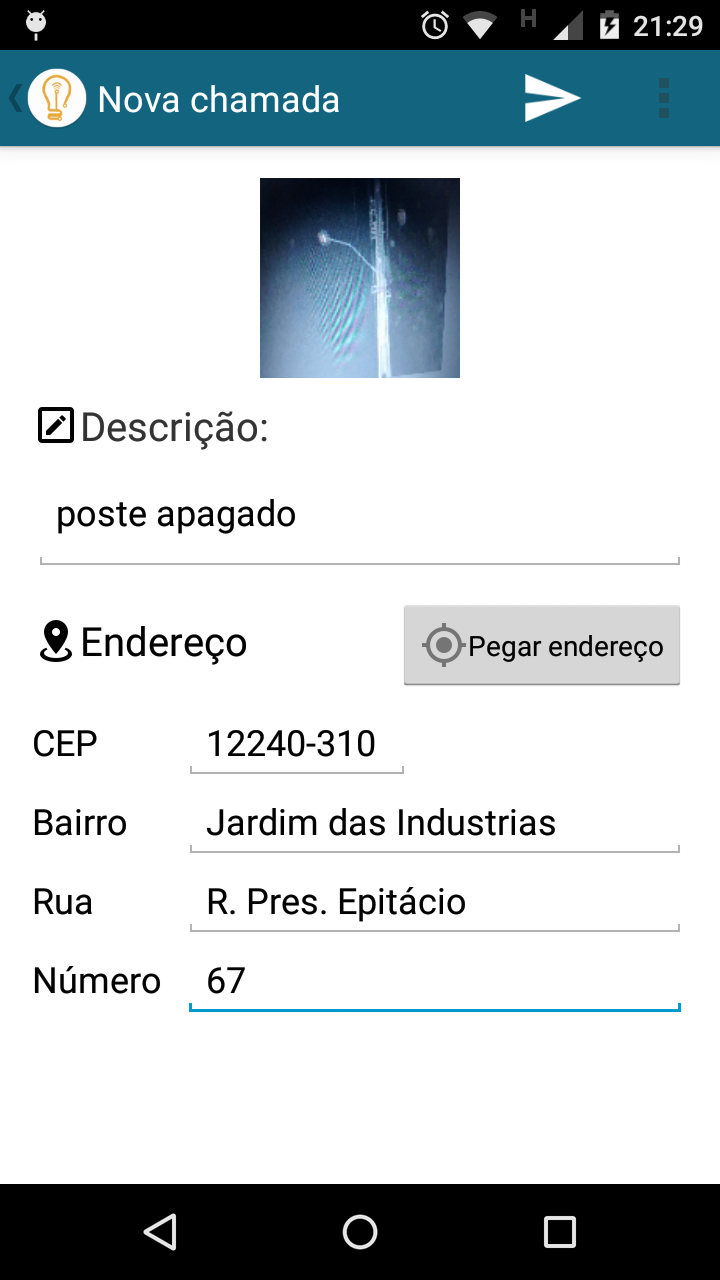
\includegraphics[scale=0.1]{android/5.png}
    \legend{Fonte: Produzido pelos autores}
  \end{minipage}
  \hfill
  \begin{minipage}{0.4\textwidth}
    \centering
    \caption{\label{android-tela-enviando}Tela de envio de protocolo com o envio em progresso}
    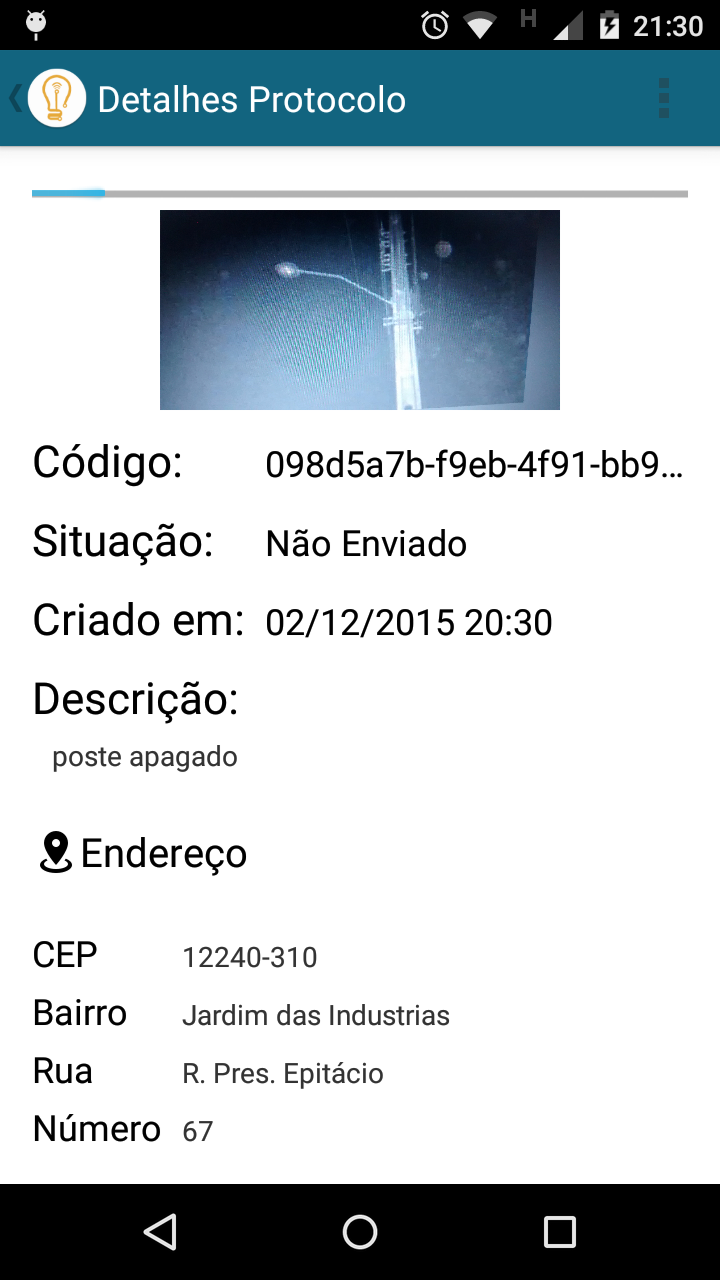
\includegraphics[scale=0.1]{android/6.png}
    \legend{Fonte: Produzido pelos autores}
  \end{minipage}
\end{figure}

Após enviado o usuário poderá escolher a opção de listar os protocolos enviados (Figura \ref{android-tela-lista-chamadas}) e checar o status do protocolo enviado (Figura \ref{android-tela-detalhes-chamada}).

\begin{figure}[!htbp]
 \centering
  \begin{minipage}{0.4\textwidth}
    \centering
    \caption{\label{android-tela-lista-chamadas}Tela de lista de protocolos feitos}
    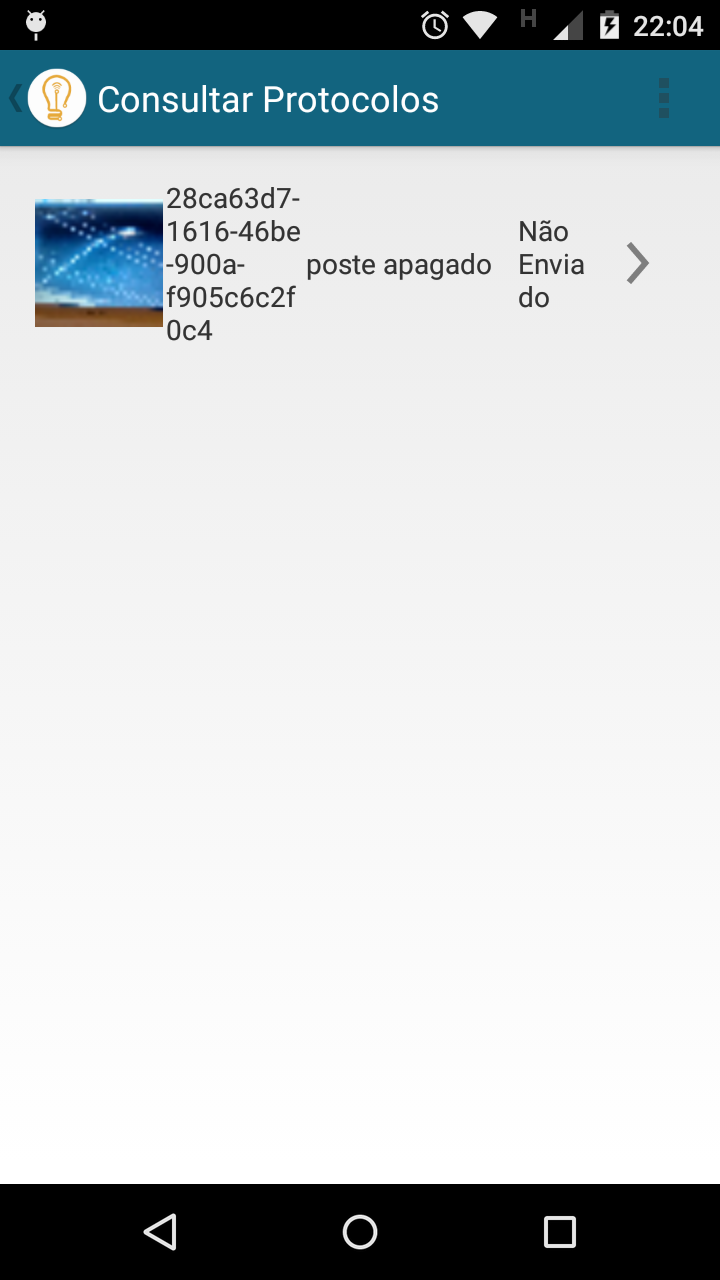
\includegraphics[scale=0.1]{android/7.png}
    \legend{Fonte: Produzido pelos autores}
  \end{minipage}
  \hfill
  \begin{minipage}{0.4\textwidth}
    \centering
    \caption{\label{android-tela-detalhes-chamada}Tela de detalhes de protocolo}
    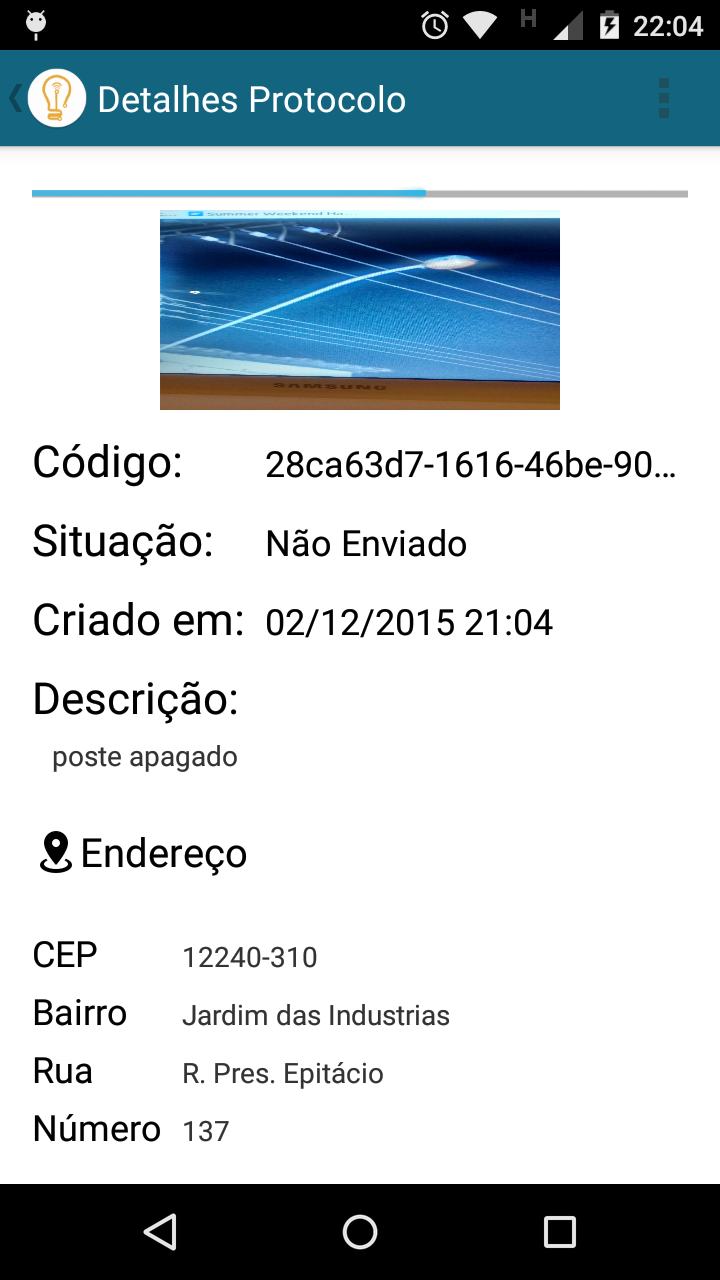
\includegraphics[scale=0.1]{android/8.png}
    \legend{Fonte: Produzido pelos autores}
  \end{minipage}
\end{figure}

O usuário também pode configurar a aplicação com o CEP padrão, e caso deseje mandar chamados em modo anônimo. Neste caso, o usuário deverá informar seu nome e e-mail para contato (Figura \ref{android-tela-preferencias}).

\begin{figure}[!htbp]
 \centering
  \begin{minipage}{0.4\textwidth}
    \centering
    \caption{\label{android-tela-preferencias}Tela de configuração de preferências}
    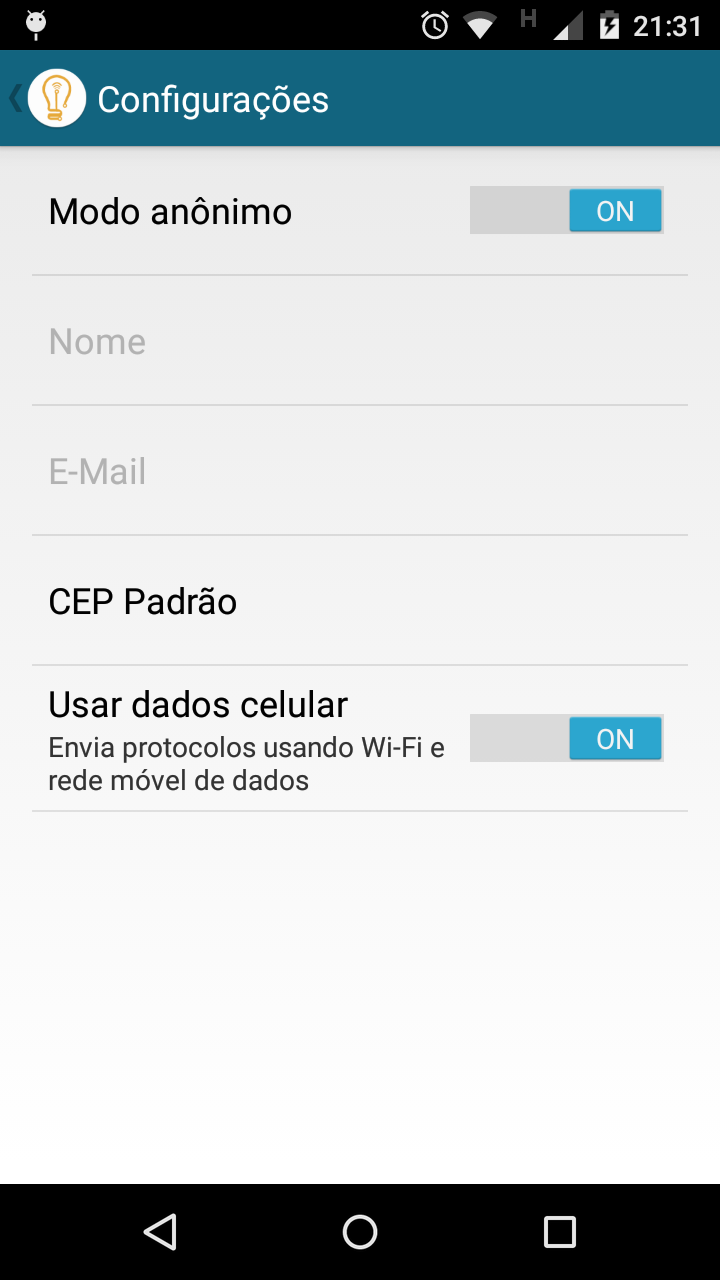
\includegraphics[scale=0.1]{android/9.png}
    \legend{Fonte: Produzido pelos autores}
  \end{minipage}
\end{figure}

\subsection{Sistema de gerenciamento de pontos de iluminação de ordens de serviço}

Como segunda fase do trabalho, foi definido que seria desenvolvido um ambiente onde os funcionários da Secretaria de Obras pudessem fazer o gerenciamento de protocolos e ordens de serviço.

\subsubsection{Entrevista inicial ao cliente}

Anteriormente a primeira entrevista, foi realizada uma apresentação do conceito do projeto para o Secretário de Obras Renê Vernice e outros integrantes da equipe.
O conceito do projeto foi não bem aceito por todos, pois a Secretaria de Obras não atenderia os chamados abertos pelo aplicativo.
Foi acordado que o projeto seguiria, caso fossem feitas algumas modificações que ajudassem na organização dos serviços realizados nos pontos de iluminação.

Posteriormente, foi feita uma reunião com a assistente do Secretário, a senhora Cintia Firmino para entendermos melhor o funcionamento do processo atual.
\begin{enumerate}

\item \textbf{Como é o processo atual?}

Processo de atualização feito a partir da coleta manual do sistema 156, e colocado numa planilha para o tratamento de pedidos duplicados e separação dos casos por zona e bairro.

\item \textbf{Como vocês recebem as chamadas dos postes com defeitos?}

Os chamados vêm do sistema 156, ou por memorando de Vereadores que tem prioridade, não possui um canal personalizado apenas para eles vem do sistema 156 (156 possui resposta programada).

\item \textbf{Como é feita a ordem de serviço?}

A ordem de serviço é feita pelo Excel, separando os chamados por zona, bairro e rua. E após isso esta planilha é enviada para a empresa URBAM por e-mail.

\item \textbf{Vocês acham que é o melhor processo? Como poderia melhorar?}

O processo poderia melhorar se os protocolos já chegassem a nós separados pela região, sem duplicidade, com a data, sem a necessidade de analisar todos os pedidos que vem do 156.

\item \textbf{Qual seria o processo ideal?}

Receber os protocolos separados pela região, bairro e rua, sem duplicidade. Responder ao munícipe automaticamente.

\item \textbf{Vocês separam os postes por tipos? Quais tipos?}

Temos dois tipos, a iluminação ornamental, e a iluminação de vias.

\item \textbf{Como vocês agrupam postes da mesma rua? Vocês têm uma base de dados de endereços?}

Os postes são agrupados em até 10 números da mesma rua. Há problemas também em verificar os endereços das praças e vielas pois tem mais de um endereço, além de algumas praças e vielas não constarem na pesquisa do Google.
Isso afeta também a troca de làmpadas ornamentais.

\item \textbf{Vocês agrupam as situações das pendências (resolvida, não resolvida, enviada para serviço, etc.)? Se não, como seria o ideal?}

Sim, por planilha, quando uma ordem de serviço e é mandada, os pedidos são retirados de uma planilha e colocadas em outra sinalizando que foram mandados e estamos esperando a resposta da URBAM.

\item \textbf{Vocês agrupam os tipos de serviços das pendências (troca de lâmpada, troca de reator, etc.)? Se não, como seria o ideal?}

Existem 3 tipos de serviços que nós justo com a URBAM, a troca de lâmpada, a troca de reator, e a troca da fotocélula.
O que será trocado é analisado um a um, pela URBAM que depois reporta o que foi trocado.

\item \textbf{Como é feita a identificação de cada poste dentro de uma rua? Pelo número aproximado da casa?}

Ainda não existe um sistema de identificação no momento.

\item \textbf{Existe algum código para identificar os postes? Se não, o código ideal deve informar o quê?}

Não existe, é pelo número da casa mais próxima ao poste.

\item \textbf{Vocês atualizam informações sobre cada ocorrência após o retorno da ordem de serviço? Se sim, o que vocês atualizam?}

Sim, a URBAM retorna uma planilha com as tarefas executadas e o que foi trocado, e após, estas informações são colocadas numa planilha chamada “Executados”, e depois é respondido para o munícipe no 156.
\end{enumerate}

\subsubsection{Requisitos do sistema CidadeIluminada}

De acordo com as respostas levantadas na reunião com a Cíntia, foram então levantados os seguintes requisitos funcionais:

\begin{description}
\item[RF1:] O sistema deverá fazer a coleta automática dos protocolos no sistema do 156 direcionados para a secretaria de obras.

\item[RF2:] O sistema deverá fazer essa coleta e, de acordo com a informação de cada protocolo, separar em bairros e regiões corretas para cada endereço.

\item[RF3:] O sistema deverá fazer a coleta sem adicionar protocolos em duplicidade.
Dois ou mais protocolos em duplicidade se caracterizam por se referirem ao
mesmo ponto de iluminação pública, tendo em vista que os postes são agrupados
logicamente de 10 em 10 metros na rua. Por exemplo, se um protocolo se referir
a um poste no número 10 da rua, e outro protocolo se referir a um poste no número
12 da rua, isso seria o mesmo poste.

\item[RF4:] O sistema deverá tentar ligar a cada protocolo a um poste, caso isso falhe, os sistemas devem permitir que o usuário faça essa correção manualmente.

\item[RF5:] O sistema deverá gerar a ordem de serviço em formato de planilha com, no máximo 50 pendências.
Na geração da ordem de serviço, o sistema deverá dar preferência em agrupar protocolos do mesmo bairro e da mesma região da cidade.

\item[RF6:] O sistema deverá permitir a atualização da situação de execução e qual foi o tipo de manutenção realizada de cada protocolo das ordens de serviço.

\item[RF7:] O sistema deverá identificar as ordens de serviço que foram executadas para que o munícipe seja alertado.

\item[RF8:] O sistema deverá permitir que se faça buscas na base de postes e protocolos.
\end{description}

\subsubsection{Fluxo de utilização do sistema de gerenciamento}

A seguir será descrito o fluxo principal de utilização do sistema de gerenciamento destinado à Secretaria Municipal de Obras de São José dos Campos.

Para iniciar, o usuário faz o login no sistema e abre o menu Protocolos onde os protocolos estão listados, como mostrado na Figura \ref{site-tela-inicial}.

\begin{figure}[!htbp]
 \centering
 \caption{\label{site-tela-inicial}Lista de protocolos}
 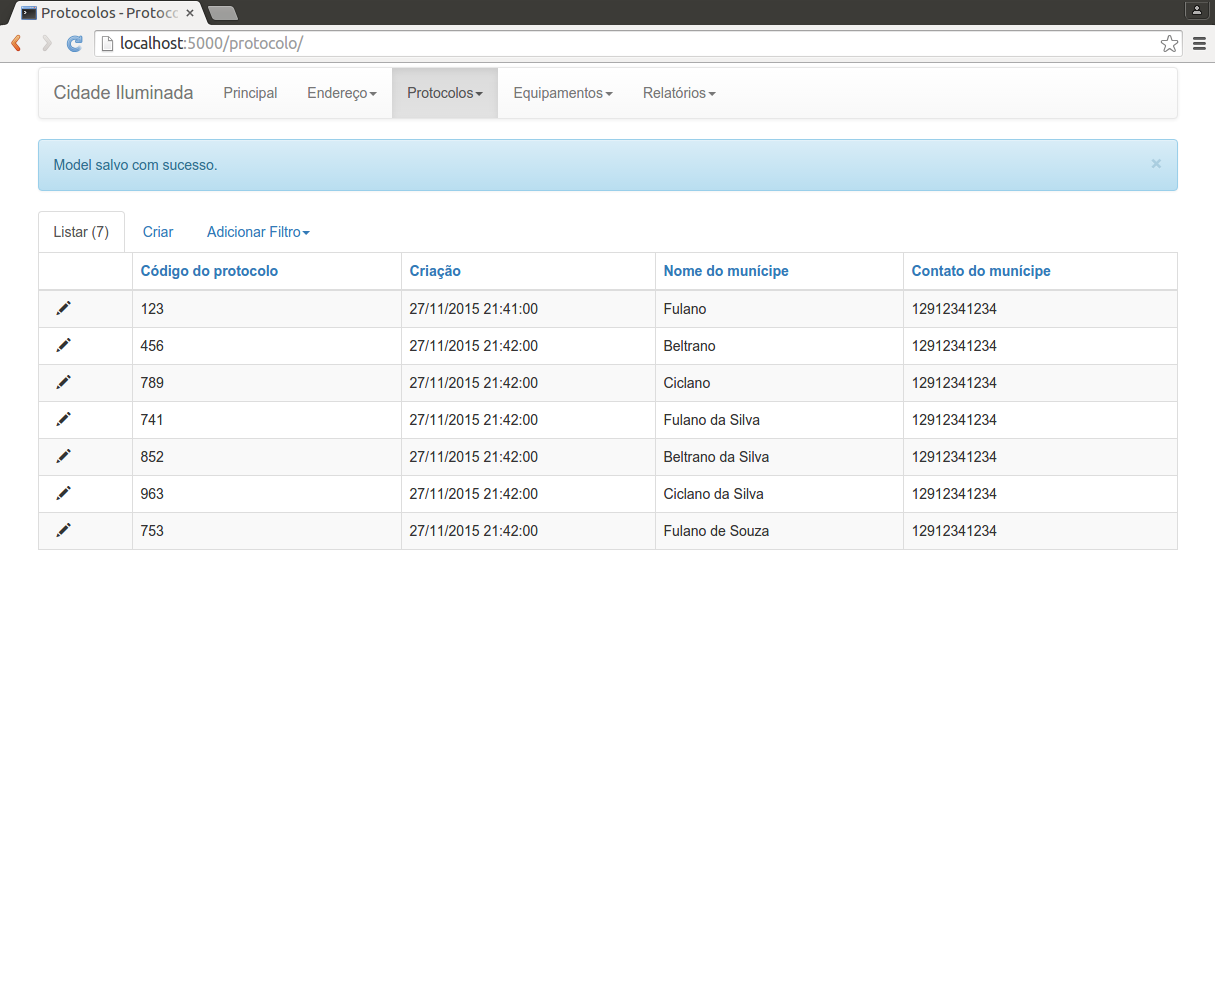
\includegraphics[scale=0.25]{site/1-lista_protocolos.png}
 \legend{Fonte: Produzido pelos autores}
\end{figure}

\clearpage

Para criar um novo protocolo, deve se clicar em Criar, onde será aberto o formulário de novo protocolo, como mostrado na Figura \ref{site-novo-protocolo}.
Note as informações necessárias para se poder criar um novo protocolo, sendo a informação mais importante qual poste que o protocolo se refere (Figura \ref{site-seleciona-poste-protocolo}).
Após a inserção, o protocolo será mostrado na lista inicial.
Para editar um protocolo, na tela da lista de protocolos (Figura \ref{site-tela-inicial}) deve-se clicar no ícone em forma de lápis, no canto esquerdo da linha do protocolo que o usuário deseja editar, e será aberto o formulário idêntico ao formulário de criação, com os dados do protocolo selecionado disponíveis para edição.

\begin{figure}[!htbp]
 \centering
 \caption{\label{site-novo-protocolo}Novo protocolo}
 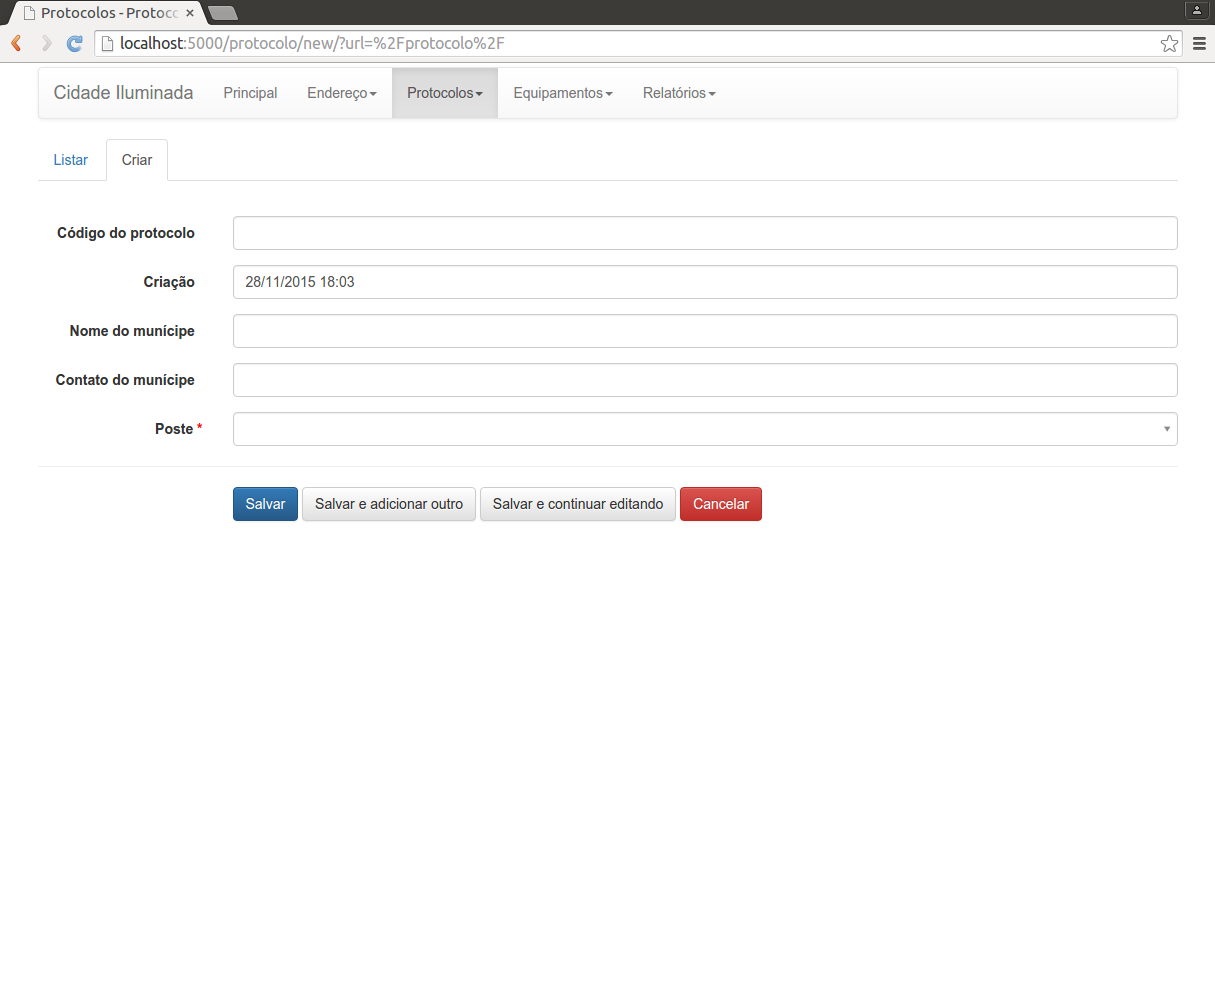
\includegraphics[scale=0.25]{site/2-novo_protocolo.png}
 \legend{Fonte: Produzido pelos autores}
\end{figure}

\begin{figure}[!htbp]
 \centering
 \caption{\label{site-seleciona-poste-protocolo}Selecionar postes}
 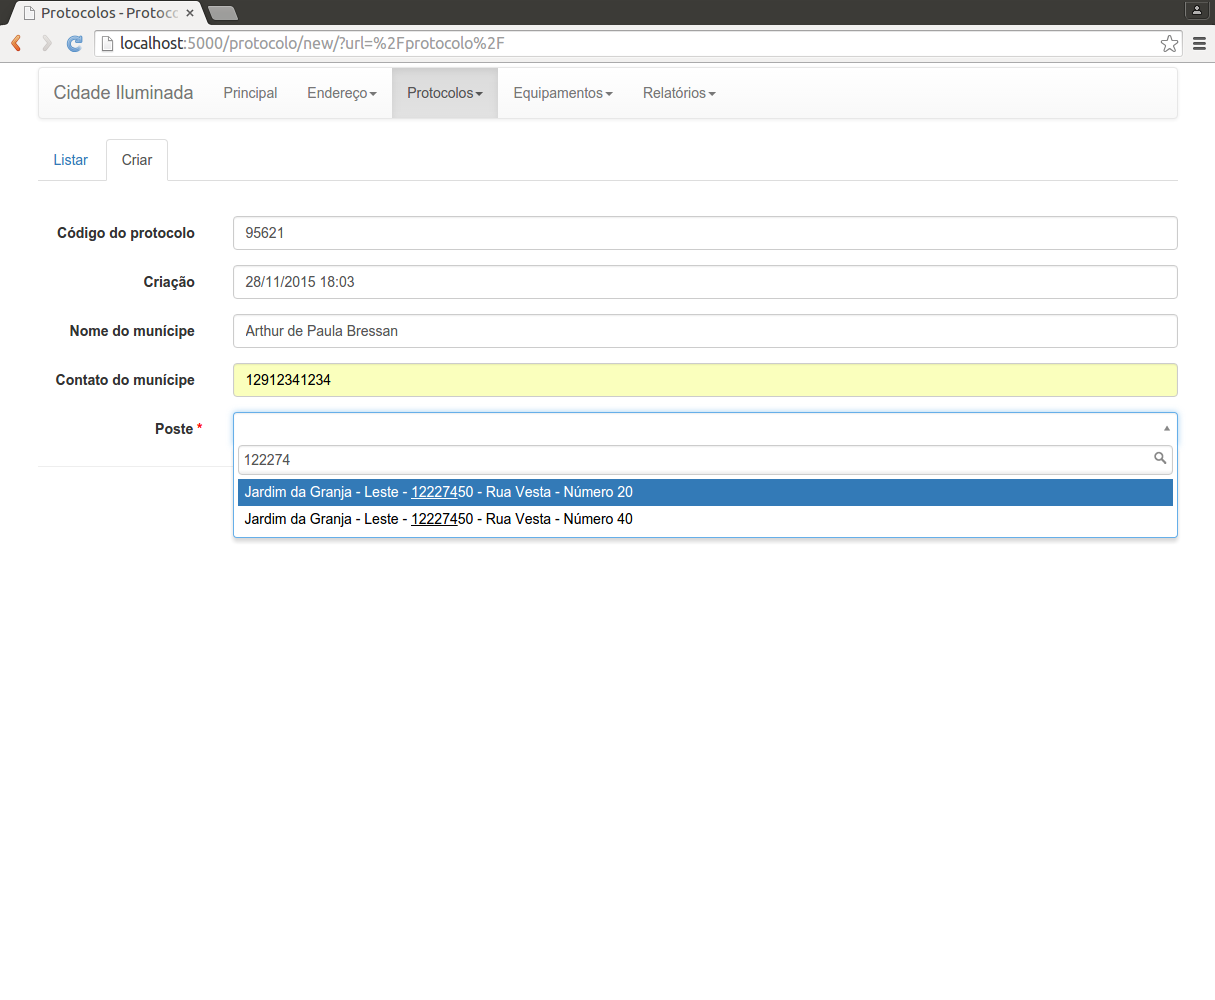
\includegraphics[scale=0.25]{site/3-seleciona_poste.png}
 \legend{Fonte: Produzido pelos autores}
\end{figure}

\clearpage

Ao associar o protocolo a um poste, essa associação pode ser confirmada através da lista de postes (Figura \ref{site-lista-poste}).

Ao selecionar o poste que se deseja ver em detalhes, é mostrado todo o seu histórico de manutenção, como mostrado na Figura \ref{site-historico-manutencao}.
A partir dessa visão, para cada item de manuteção do poste, pode estar associado um ou vários protocolos, como por exemplo na Figura \ref{site-protocolos-poste}.

\begin{figure}[!htbp]
 \centering
 \caption{\label{site-lista-poste}Lista de postes}
 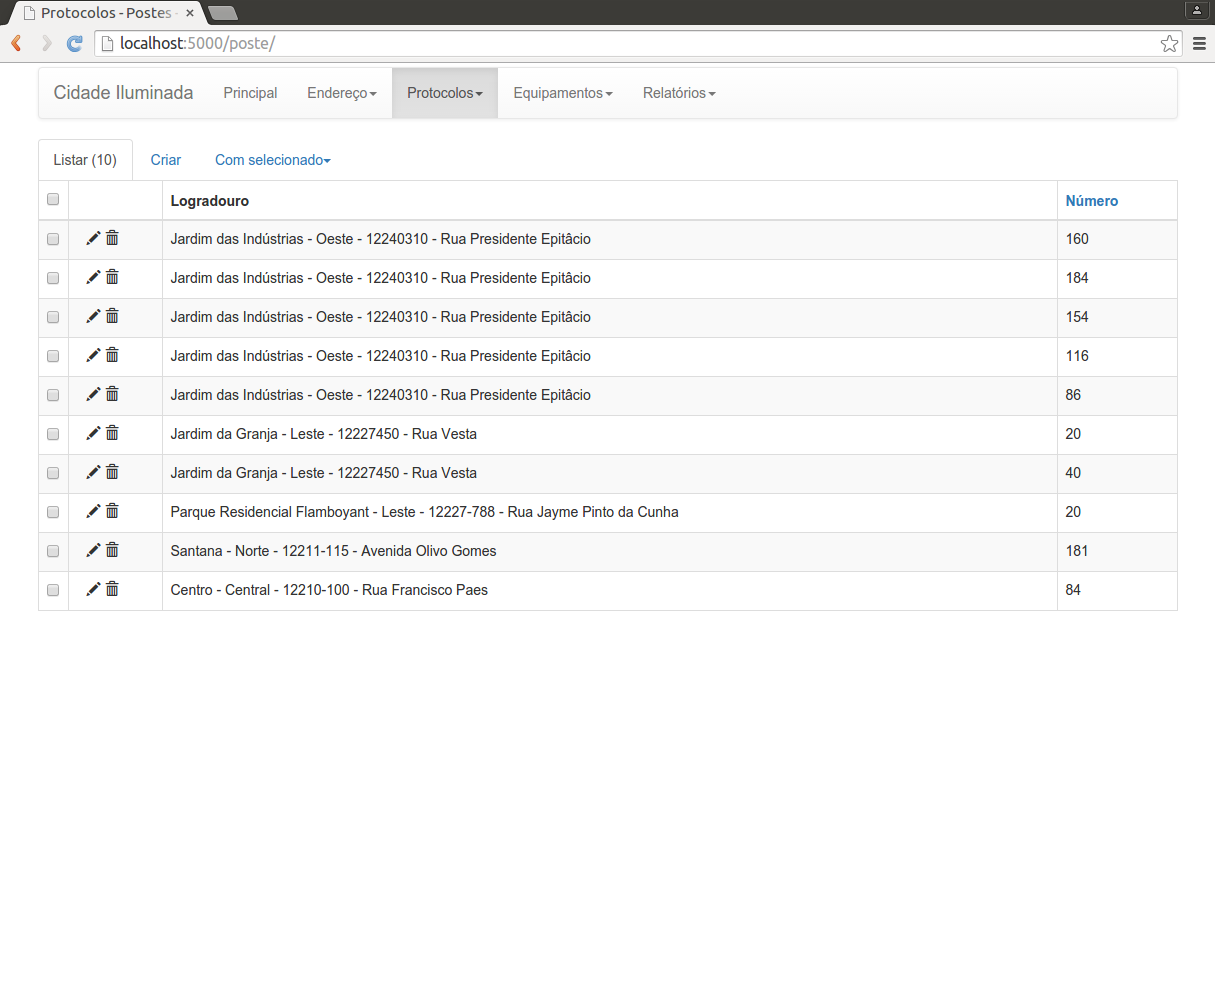
\includegraphics[scale=0.25]{site/4-lista_postes.png}
 \legend{Fonte: Produzido pelos autores}
\end{figure}

\begin{figure}[!htbp]
 \centering
 \caption{\label{site-historico-manutencao}Histórico de manutenção do poste}
 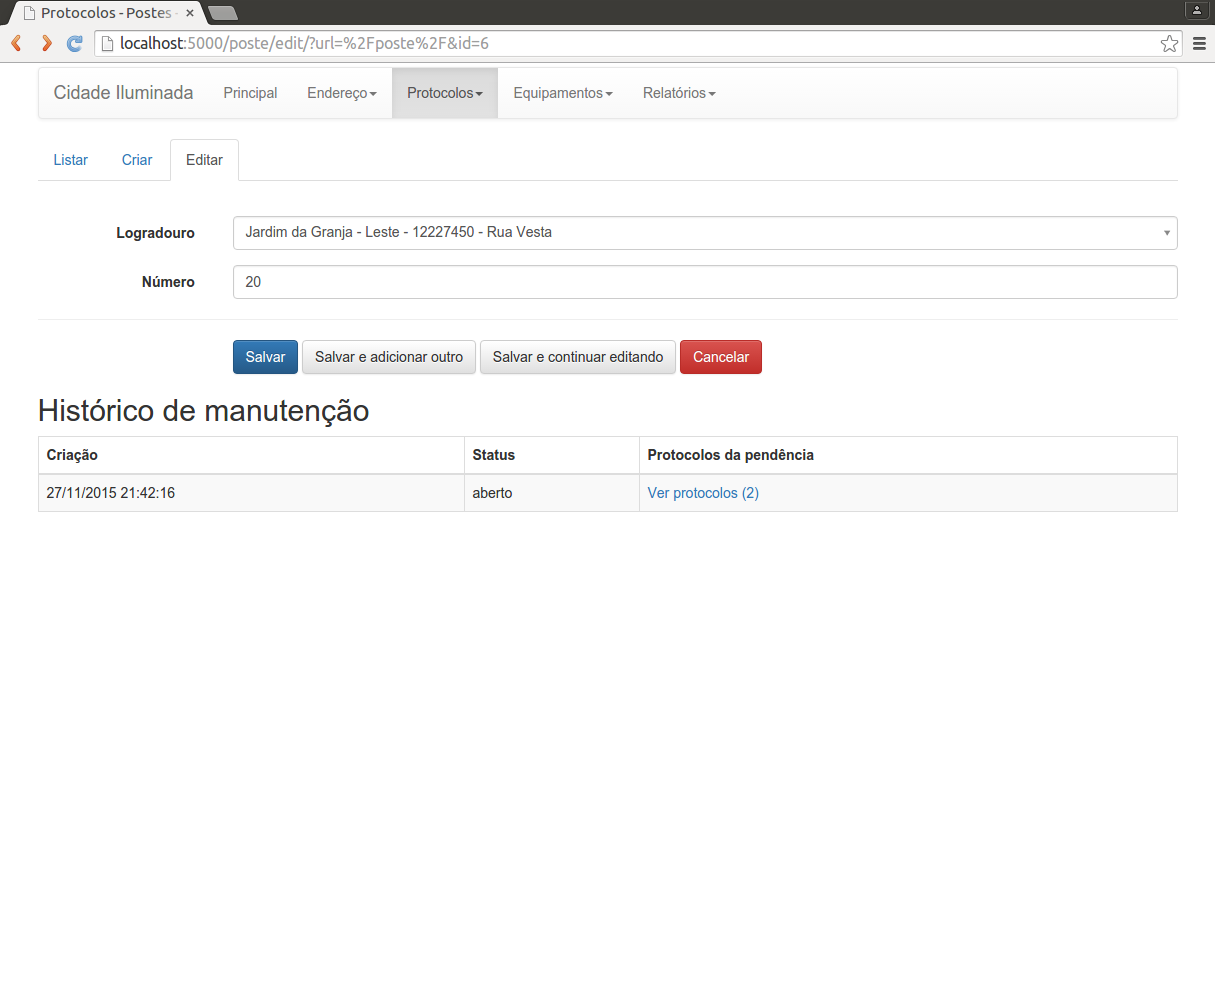
\includegraphics[scale=0.25]{site/5-historico_manutencao_poste.png}
 \legend{Fonte: Produzido pelos autores}
\end{figure}

\begin{figure}[!htbp]
 \centering
 \caption{\label{site-protocolos-poste}Protocolos associados ao poste}
 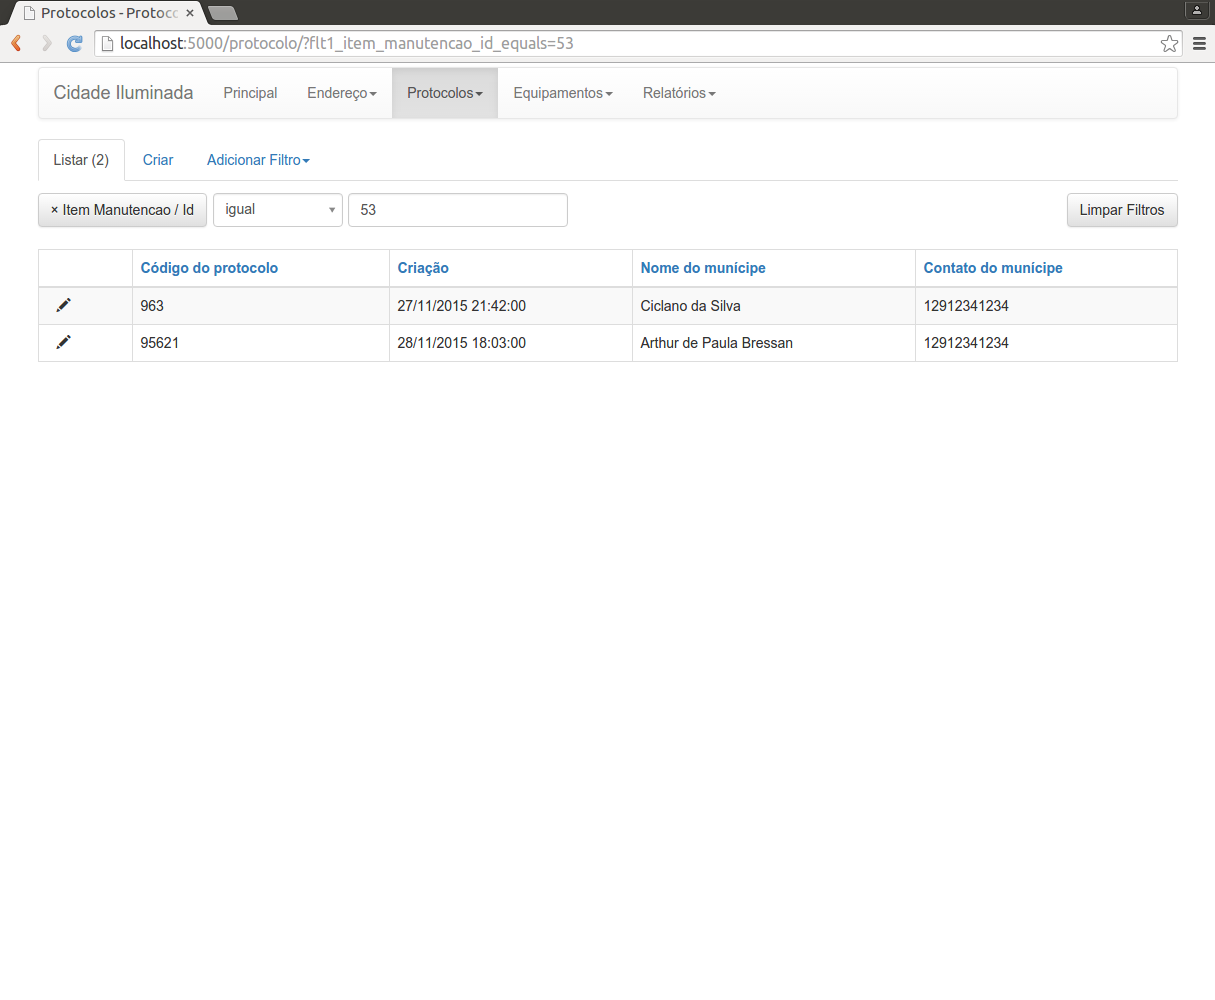
\includegraphics[scale=0.25]{site/6-protocolos_poste.png}
 \legend{Fonte: Produzido pelos autores}
\end{figure}

\clearpage

Para o usuário da Secretaria de Obras, no menu Principal é possível visualizar as Ordens de Serviço em aberto e também gerar novas Ordens de Serviço, como pode ser visto na Figura \ref{site-tela-secretaria}.

Para gerar uma nova Ordem de Serviço, o usuário deverá clicar na região desejada, selecionar os bairros (Figura \ref{site-seleciona-bairro}) e, por fim, confirmar os postes com pendências, como mostrado na Figura \ref{site-seleciona-poste-ordem-servico}.

Após selecionar todos os postes com pendências que se deseja adicionar na nova Ordem de Serviço, a Ordem de Serviço pode então ser finalmente criada ao clicar no botão de Gerar Ordem de Serviço.
Assim uma nova Ordem de Serviço é gerada como mostrado na Figura \ref{site-os-gerada}.

\begin{figure}[!htbp]
 \centering
 \caption{\label{site-tela-secretaria}Tela principal da secretaria}
 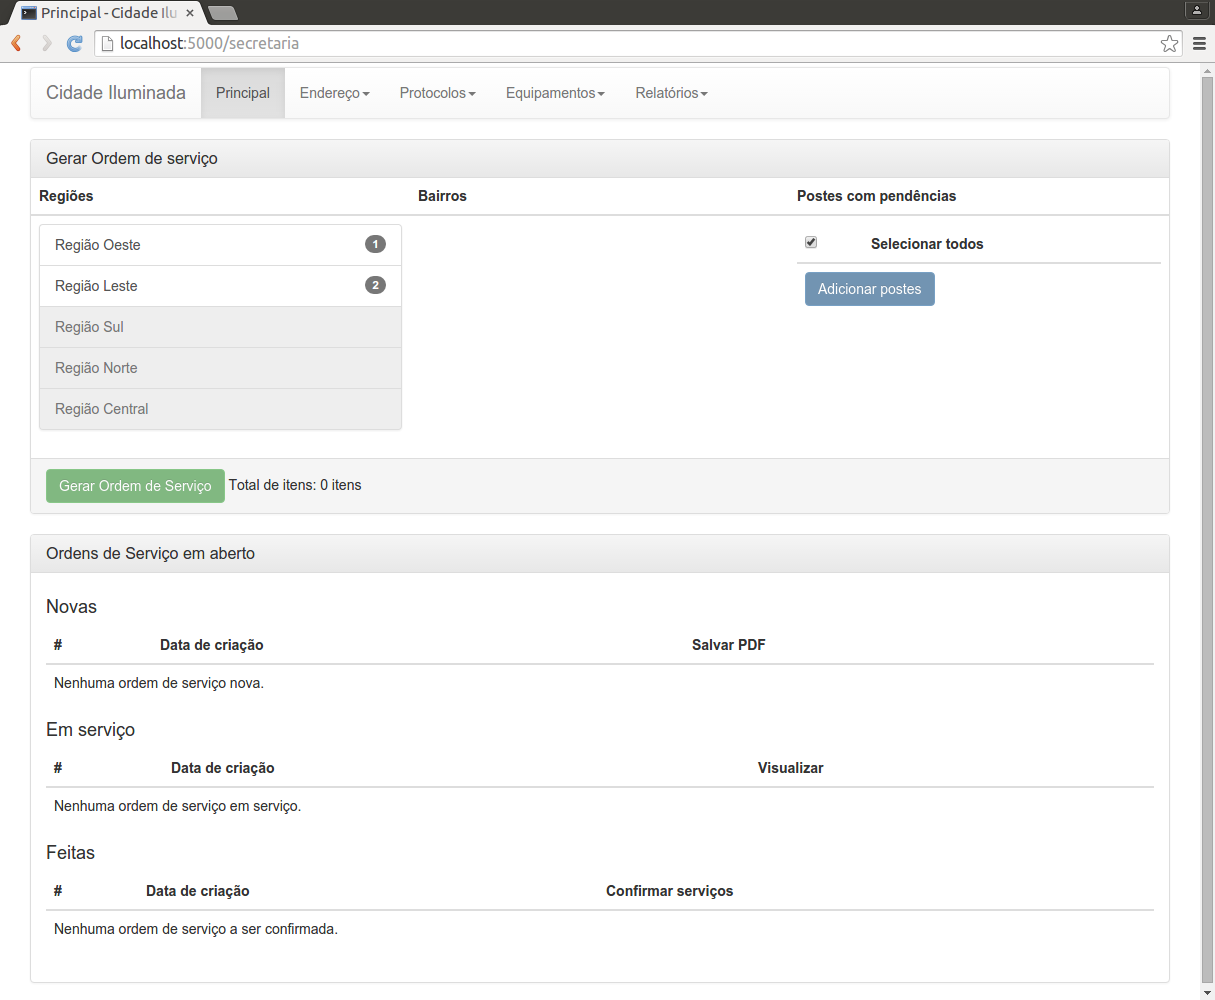
\includegraphics[scale=0.25]{site/7-tela_secretaria.png}
 \legend{Fonte: Produzido pelos autores}
\end{figure}

\begin{figure}[!htbp]
 \centering
 \caption{\label{site-seleciona-bairro}Tela principal da secretaria com a região e bairro selecionado}
 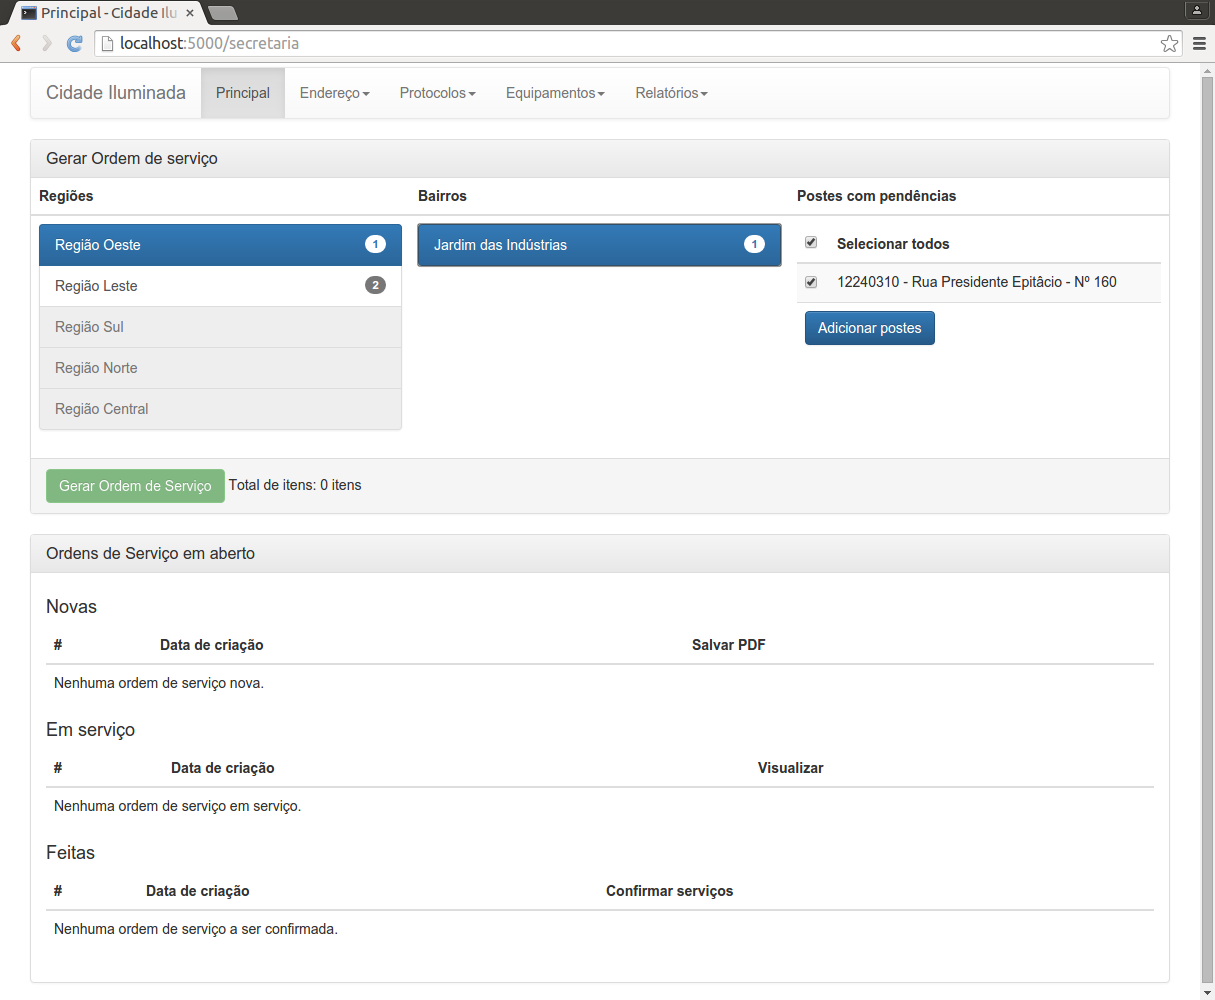
\includegraphics[scale=0.25]{site/8-bairro.png}
 \legend{Fonte: Produzido pelos autores}
\end{figure}

\begin{figure}[!htbp]
 \centering
 \caption{\label{site-seleciona-poste-ordem-servico}Postes da região oeste selecionados}
 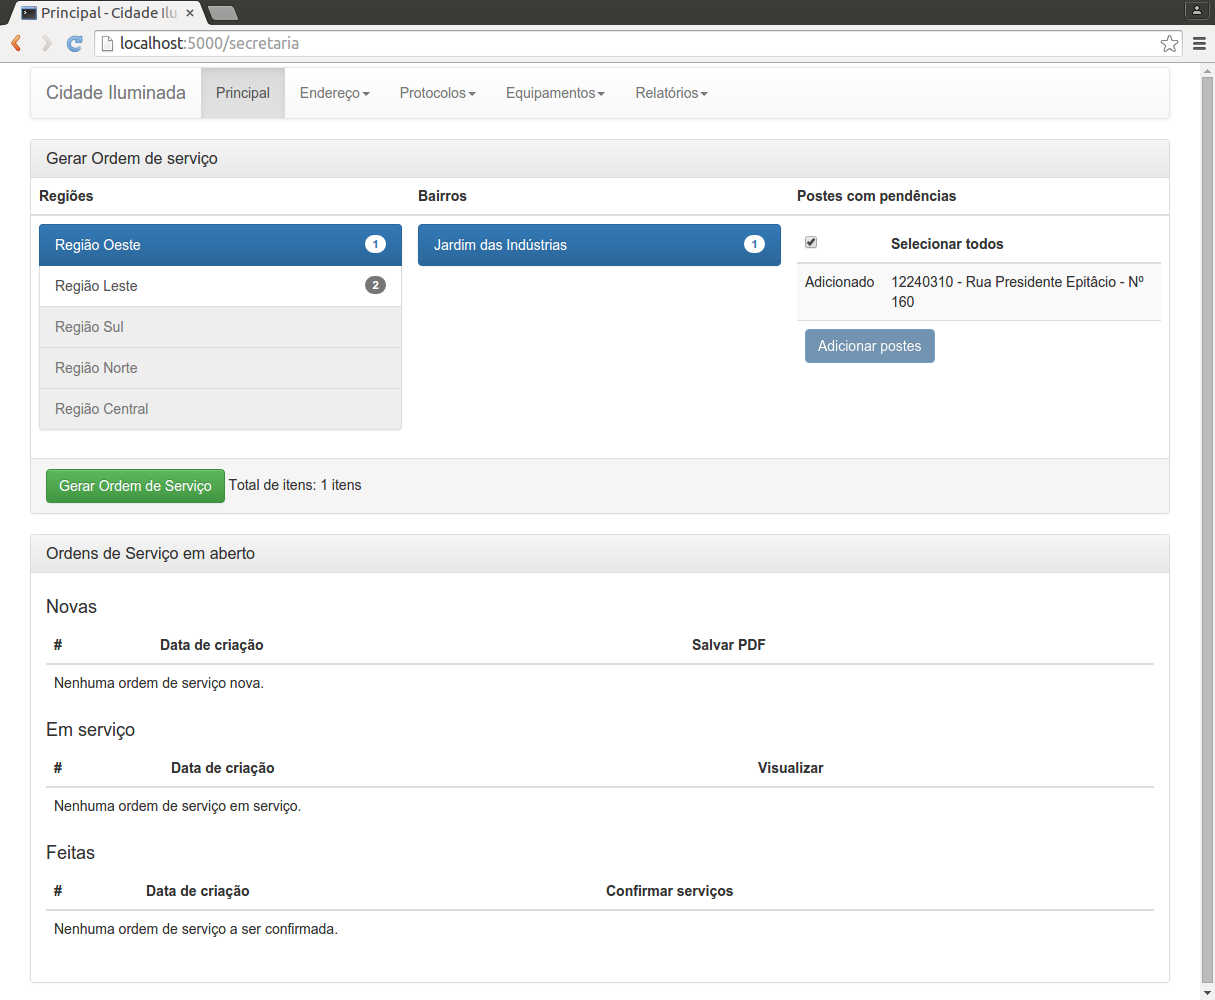
\includegraphics[scale=0.25]{site/9-poste_selecionado.png}
 \legend{Fonte: Produzido pelos autores}
\end{figure}

\begin{figure}[!htbp]
 \centering
 \caption{\label{site-os-gerada}Ordem de Serviço gerada}
 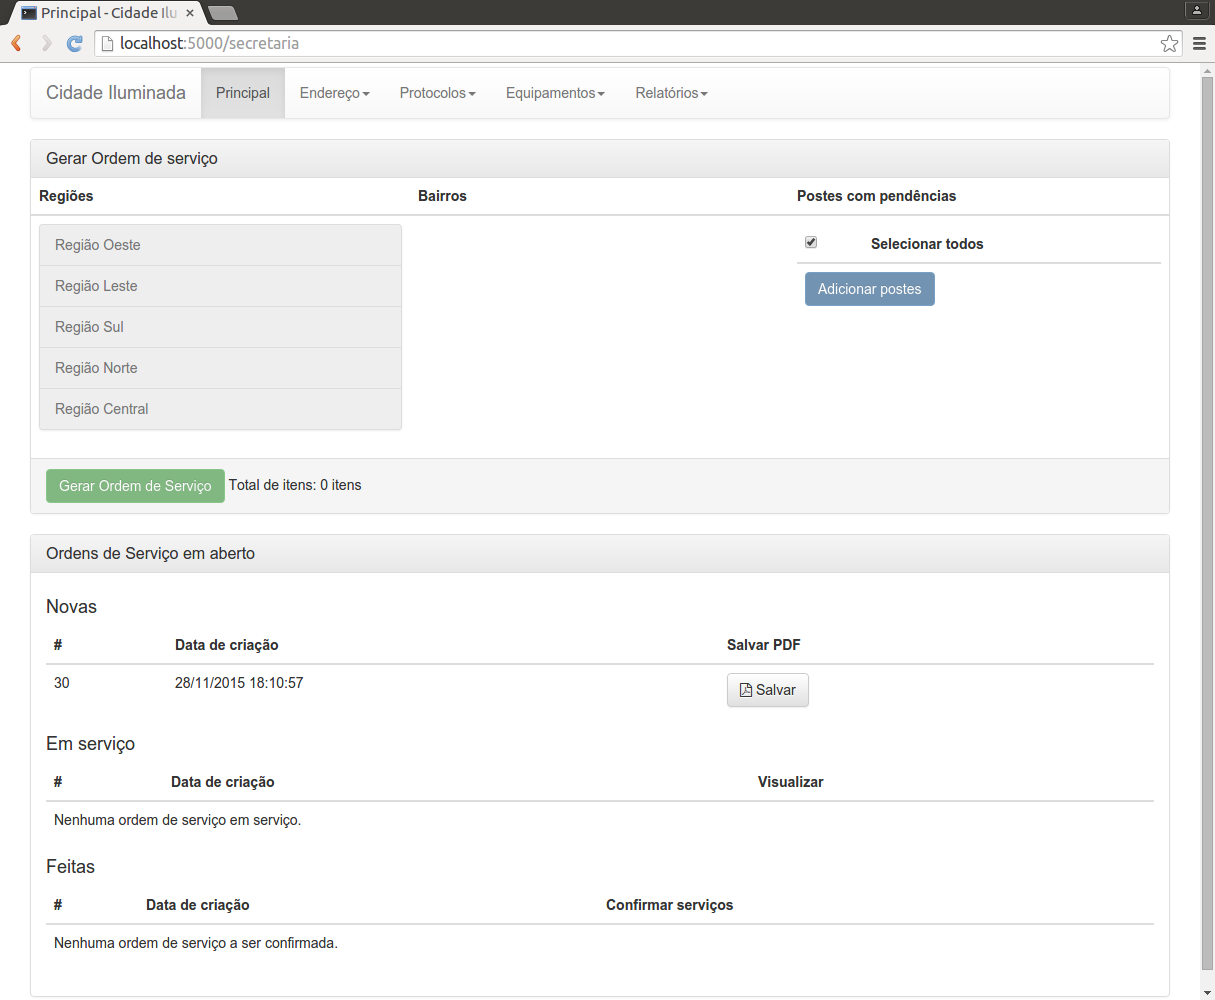
\includegraphics[scale=0.25]{site/11-os_gerada.png}
 \legend{Fonte: Produzido pelos autores}
\end{figure}

\clearpage

Tanto o usuário da Secretaria de Obras quanto o usuário da URBAM tem acesso ao PDF que será gerado, como mostrado na Figura \ref{site-pdf}.
A finalidade do PDF é servir como apoio em campo para os operários da URBAM para melhor relatarem os serviços feitos e equipamentos utilizados.
Esse PDF mostra uma grade com o endereço completo dos postes da Ordem de Serviço, bem como os equipamentos previamente cadastrados que podem ser utilizados.
Além disso, esta grade possui um campo para o preenchimento do motivo de não realização do serviço, caso seja necessário.

\begin{figure}[!htbp]
 \centering
 \caption{\label{site-pdf}Lista de serviços da Ordem de Serviço}
 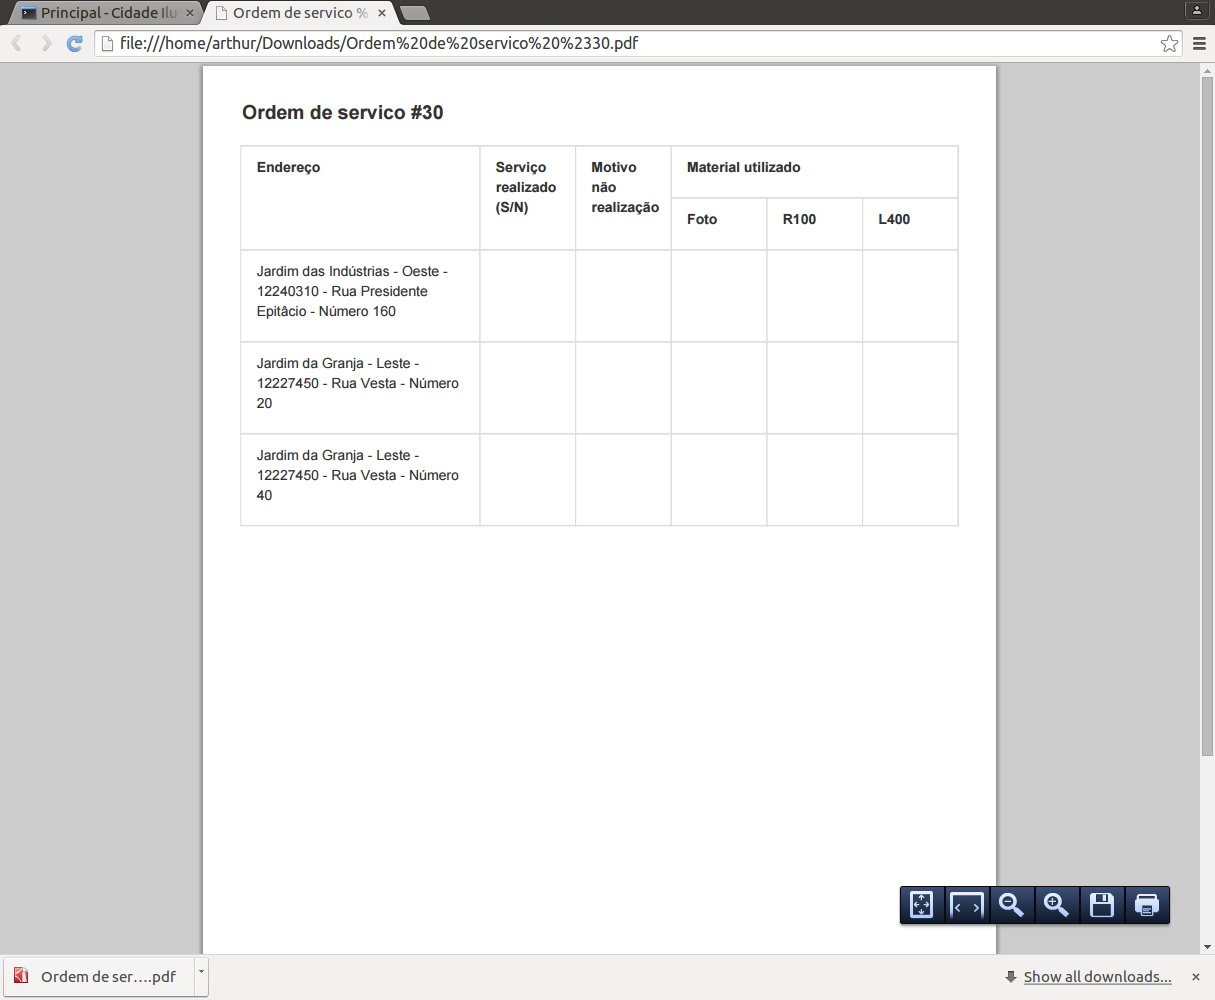
\includegraphics[scale=0.25]{site/12-pdf.png}
 \legend{Fonte: Produzido pelos autores}
\end{figure}

\clearpage

Assim que uma equipe de manutenção for despachada, o usuário da URBAM (Figura \ref{site-visao-urbam}) deverá sinalizar este envio clicando no botão Enviar para serviço.
Após isso, a Ordem de Serviço irá mudar de status para Em serviço, e estará disponível para que seja realizado o seu eventual fechamento (Figura \ref{site-servico-os}).

\begin{figure}[!htbp]
 \centering
 \caption{\label{site-visao-urbam}Tela principal do usuário da URBAM}
 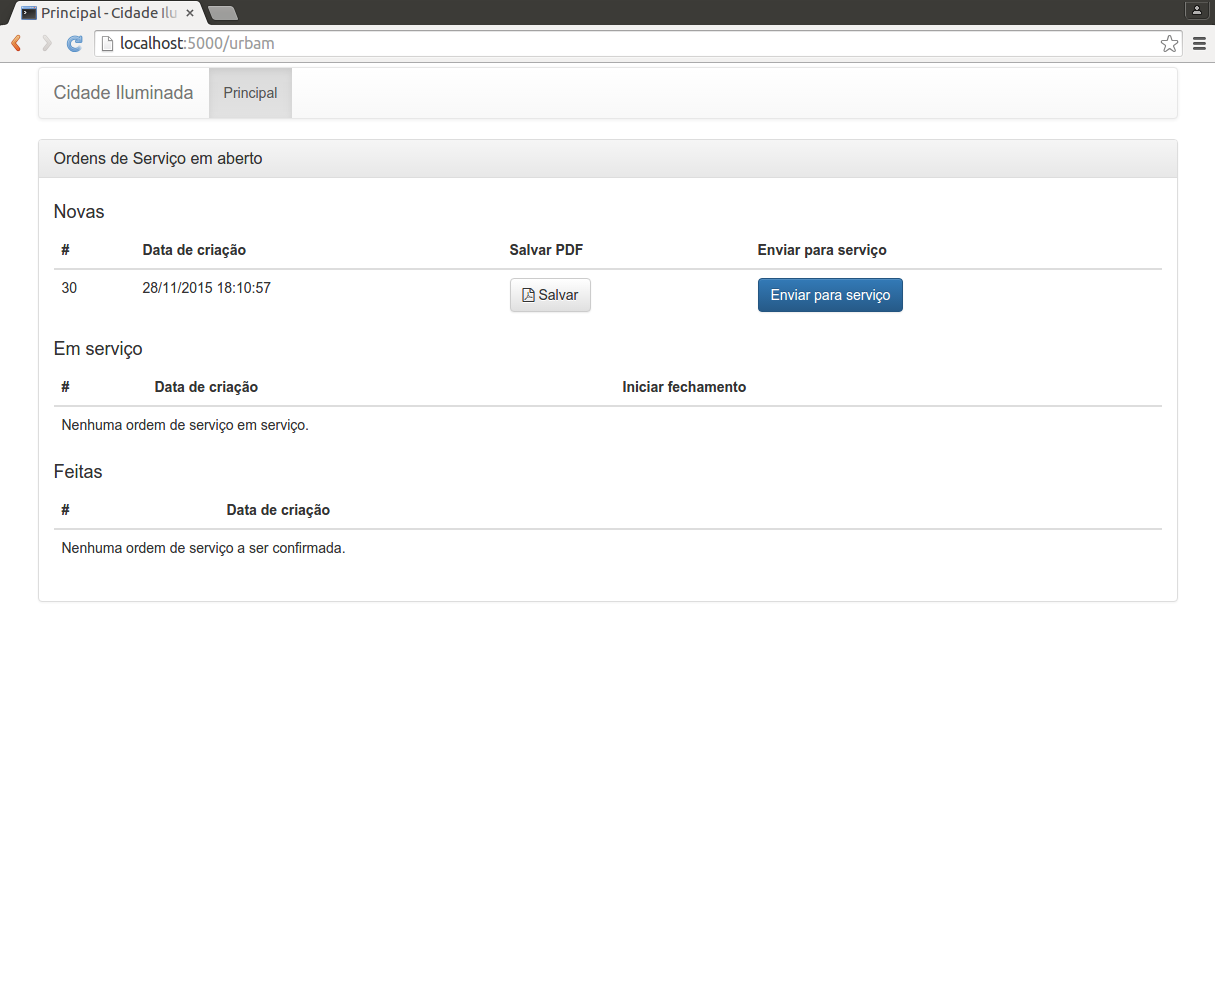
\includegraphics[scale=0.25]{site/13-urbam.png}
 \legend{Fonte: Produzido pelos autores}
\end{figure}

\begin{figure}[!htbp]
 \centering
 \caption{\label{site-servico-os}Ordem de Serviço sinalizada como Em serviço}
 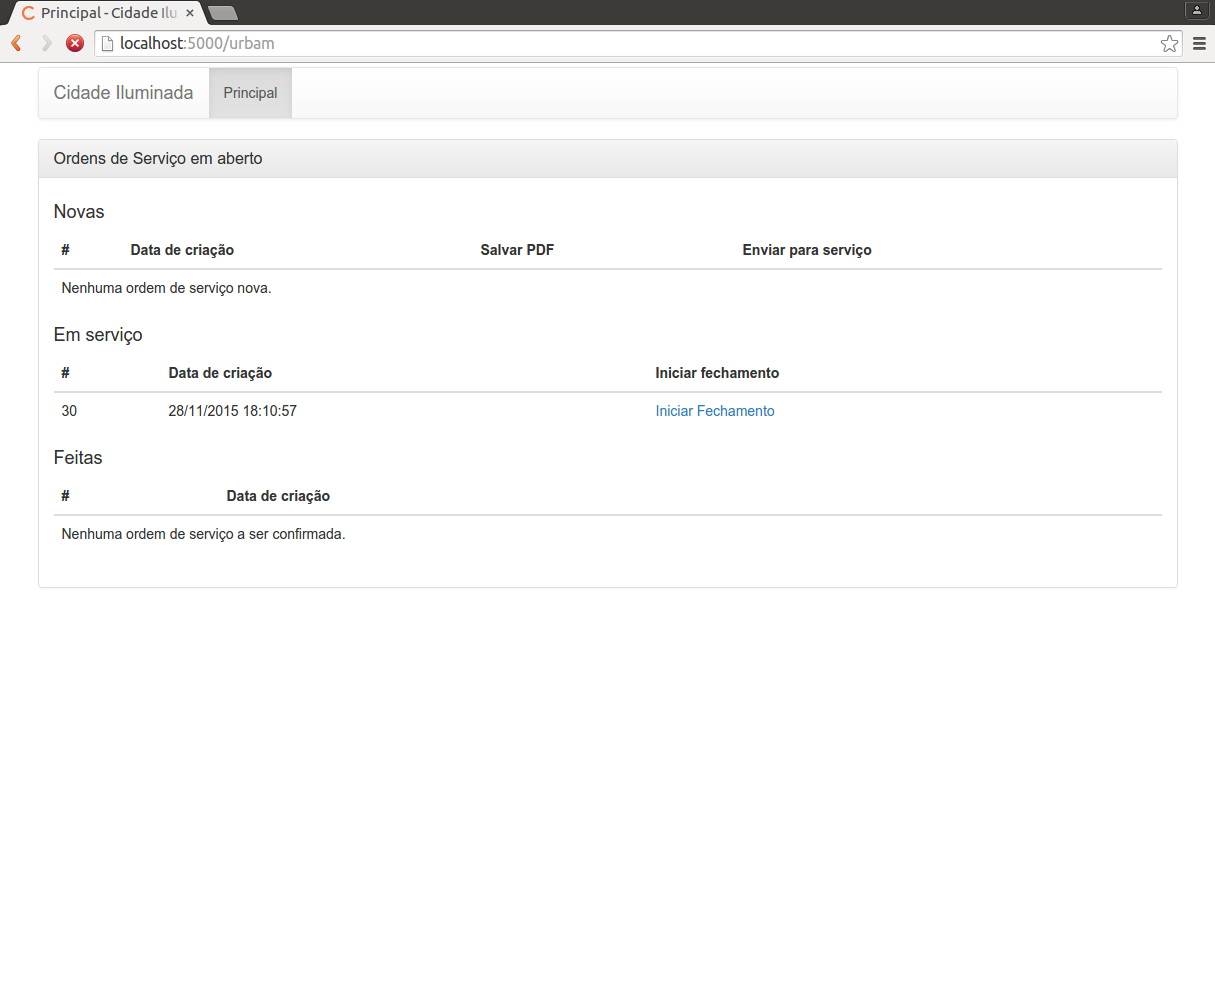
\includegraphics[scale=0.25]{site/14-servico_os.png}
 \legend{Fonte: Produzido pelos autores}
\end{figure}

\clearpage

Para fechar uma Ordem de Serviço em aberto, o usuário da URBAM deverá clicar em Iniciar Fechamento, e então o usuário será redirecionado para a tela de fechamento (Figura \ref{site-fechamento-urbam}).
Neste momento, etapa o usuário irá informar ao sistema se o serviço foi realizado, e o material utilizado, como a Figura \ref{site-material-e-motivo} mostra.
Após o fechamento de todos os serviços, o status da Ordem de Serviço ficará como Feita, ilustrado na Figura \ref{site-os-feita}.

\begin{figure}[!htbp]
 \centering
 \caption{\label{site-fechamento-urbam}Tela de fechamento de serviço da URBAM}
 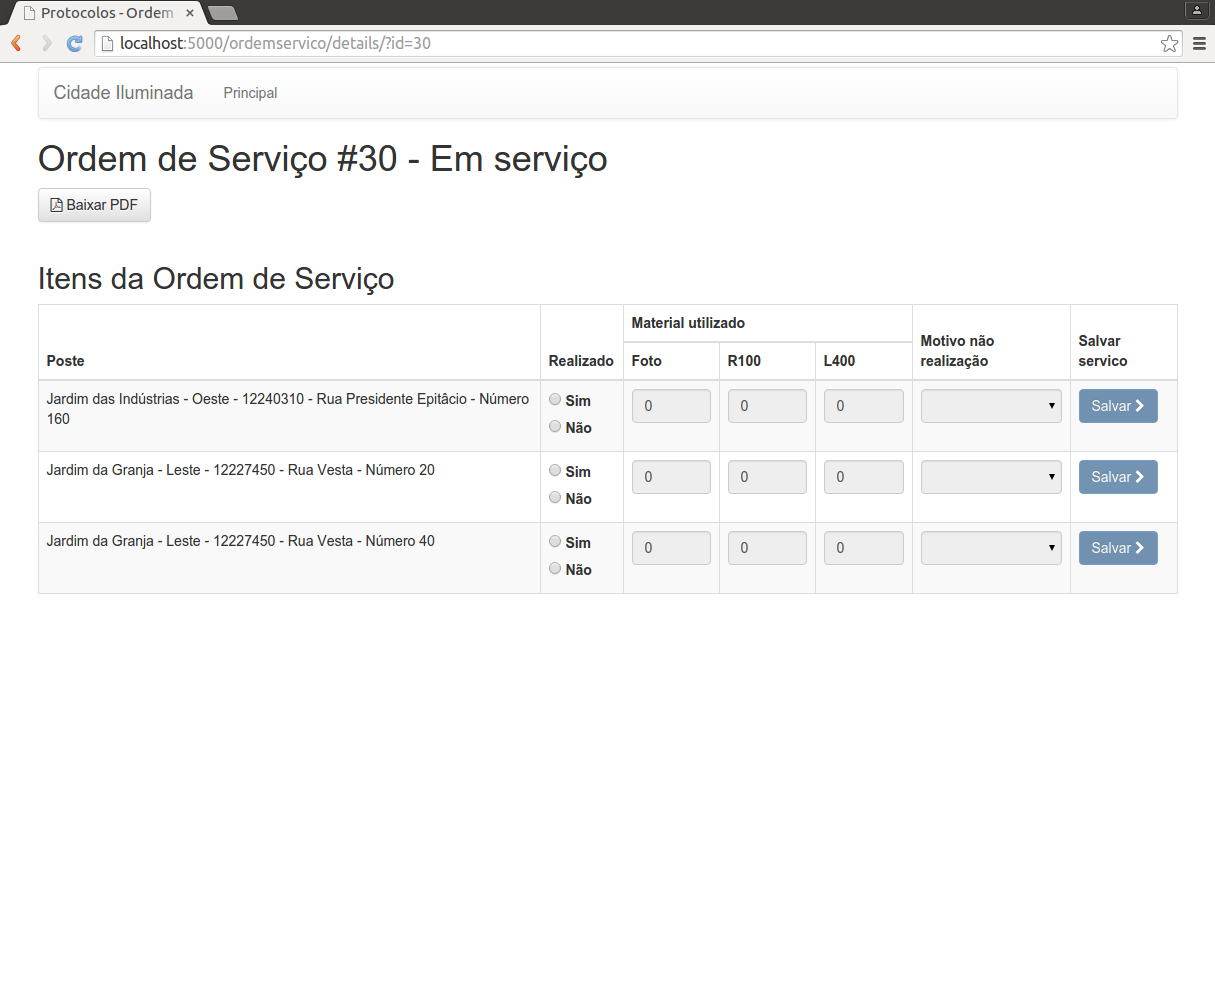
\includegraphics[scale=0.25]{site/15-fechamento_urbam.png}
 \legend{Fonte: Produzido pelos autores}
\end{figure}

\begin{figure}[!htbp]
 \centering
 \caption{\label{site-material-e-motivo}Tela de fechamento preenchida}
 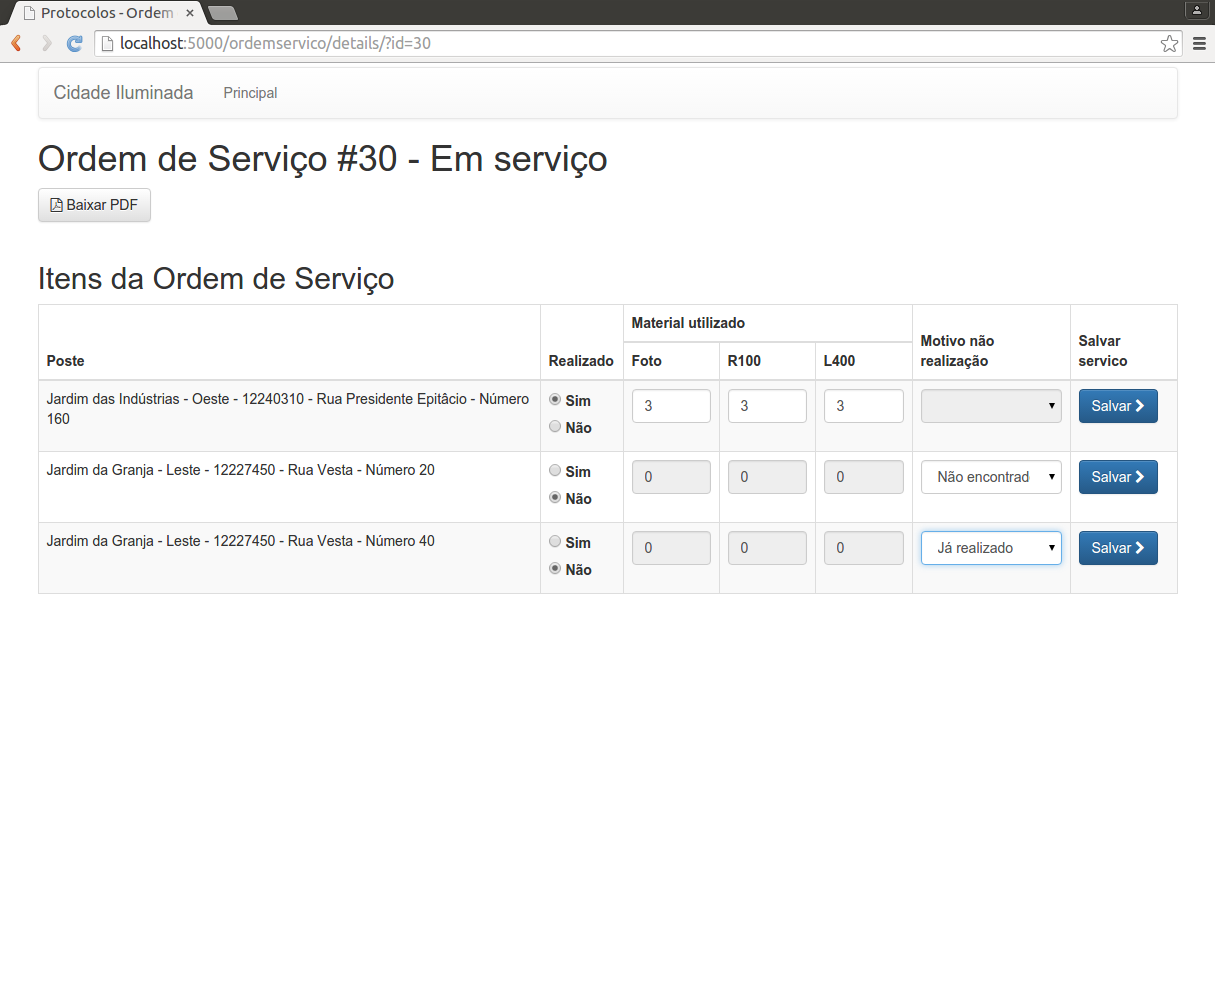
\includegraphics[scale=0.25]{site/16-material_e_motivo.png}
 \legend{Fonte: Produzido pelos autores}
\end{figure}

\begin{figure}[!htbp]
 \centering
 \caption{\label{site-os-feita}Ordem de Serviço feita}
 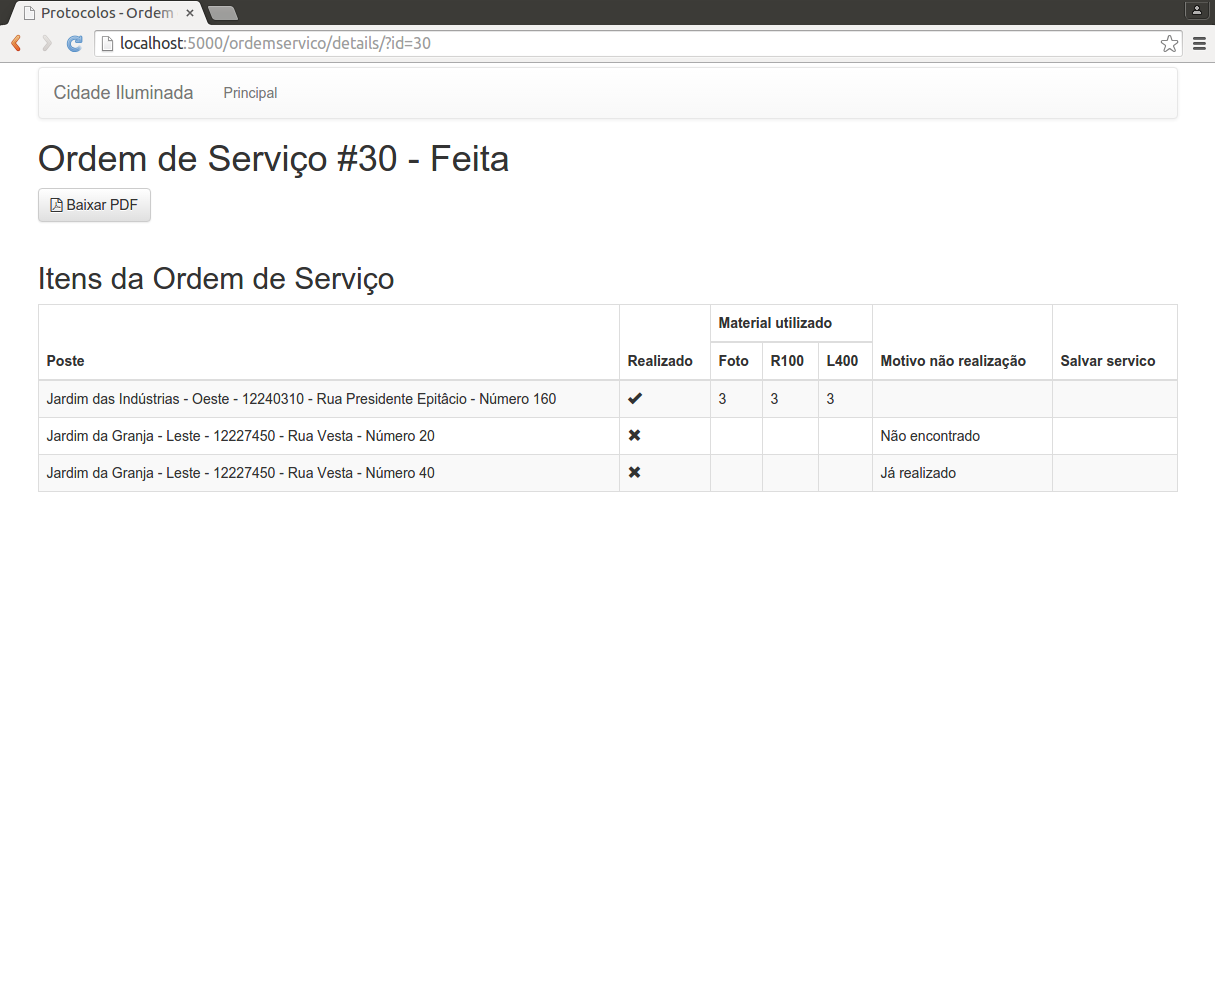
\includegraphics[scale=0.25]{site/17-os_feita.png}
 \legend{Fonte: Produzido pelos autores}
\end{figure}

\clearpage

Com a Ordem de Serviço Feita, o usuário da Secretaria deve confirmar o material utilizado em cada serviço realizado, além de conferir o motivo de alguns dos serviços não terem sido executados.

Para confirmar uma Ordem de Serviço, o usuário da Secretaria deve abrir a página principal e procurar na lista de Ordens de Serviço Feitas a Ordem de Serviço que se deseja confirmar e clicar no link de Confirmar Serviços (Figura \ref{site-os-confirmacao}).

Após isso, irá ser aberta uma tela similar à tela de fechamento de serviço da URBAM. Porém, para cada serviço irá ser mostrado o material utilizado ou o motivo de não realização do serviço (Figura \ref{site-os-confirmando}), um campo para o comentário por parte da Secretaria e um botão para confirmar o serviço.

Assim que a Ordem de Serviço tiver com todos os serviços confirmados, a sua situação irá mudar para Feita, o que sinaliza que não é necessário mais nenhuma ação (Figura \ref{site-os-confirmada}).

\begin{figure}[!htbp]
 \centering
 \caption{\label{site-os-confirmacao}Lista de Ordem de Serviço feitas}
 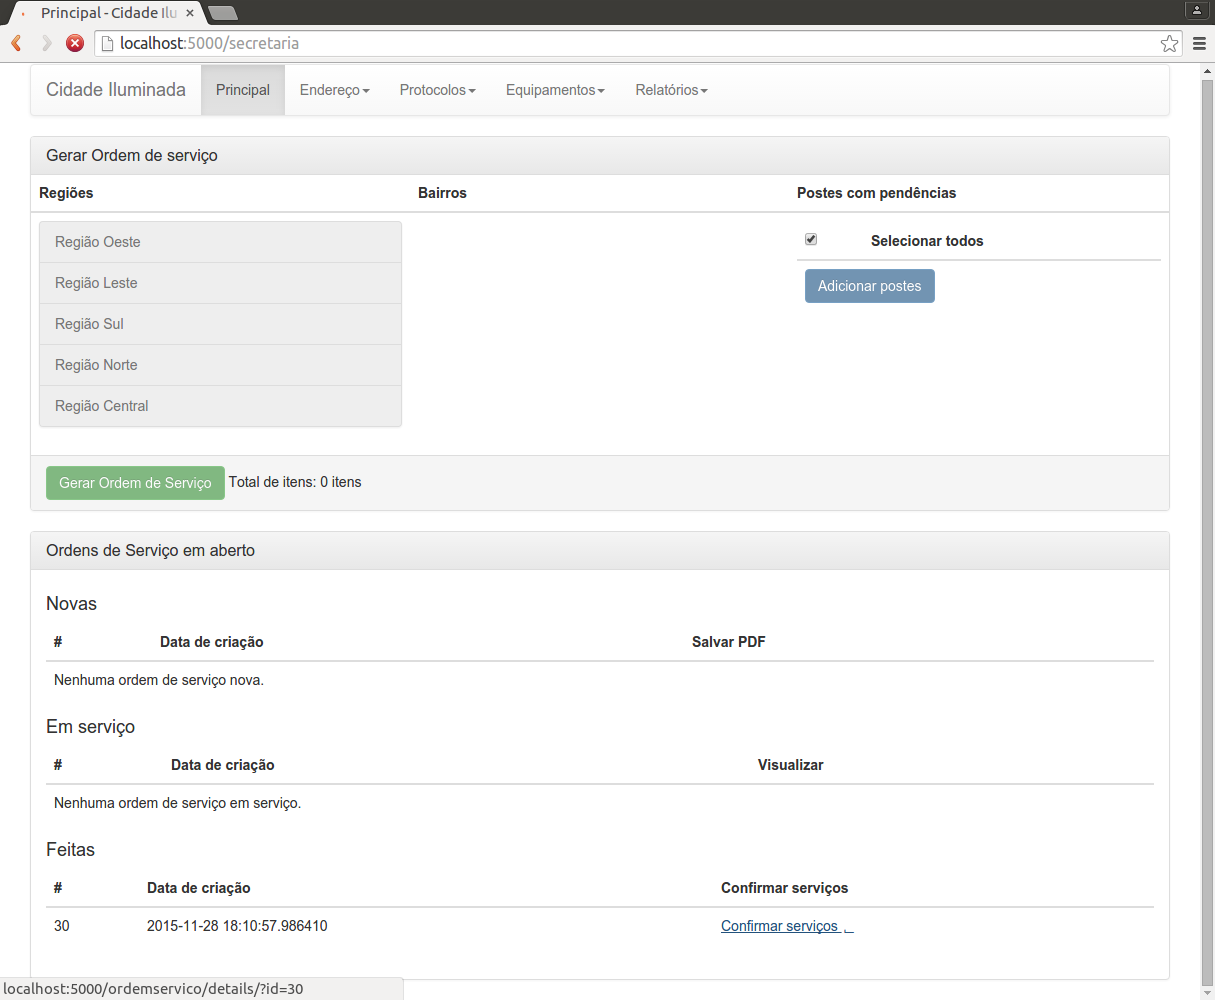
\includegraphics[scale=0.25]{site/18-os_confirmacao.png}
 \legend{Fonte: Produzido pelos autores}
\end{figure}

\begin{figure}[!htbp]
 \centering
 \caption{\label{site-os-confirmando}Confirmação da Ordem de Serviço}
 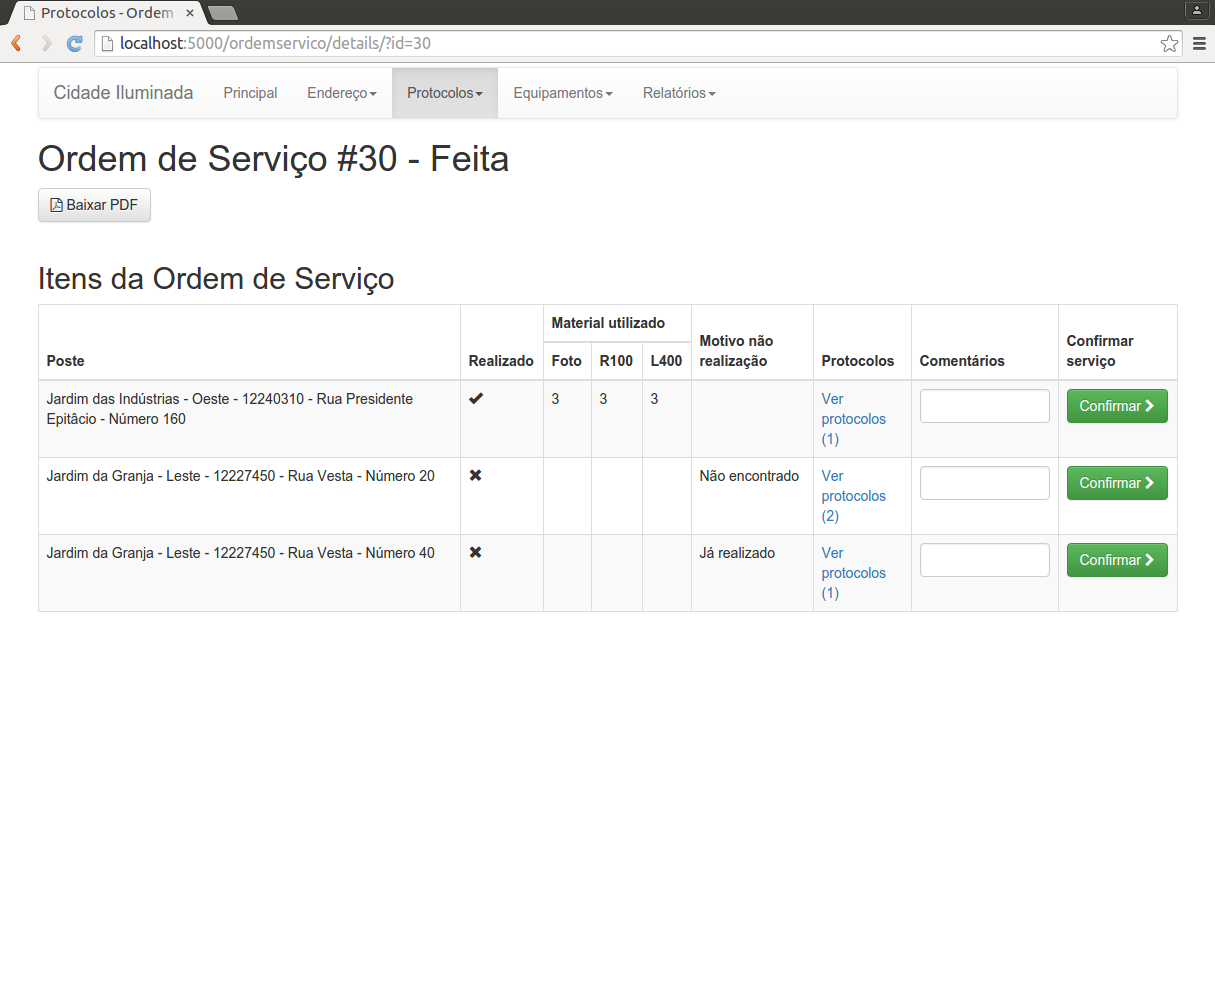
\includegraphics[scale=0.25]{site/19-os_confirmando.png}
 \legend{Fonte: Produzido pelos autores}
\end{figure}

\begin{figure}[!htbp]
 \centering
 \caption{\label{site-os-confirmada}Ordem de Serviço confirmada}
 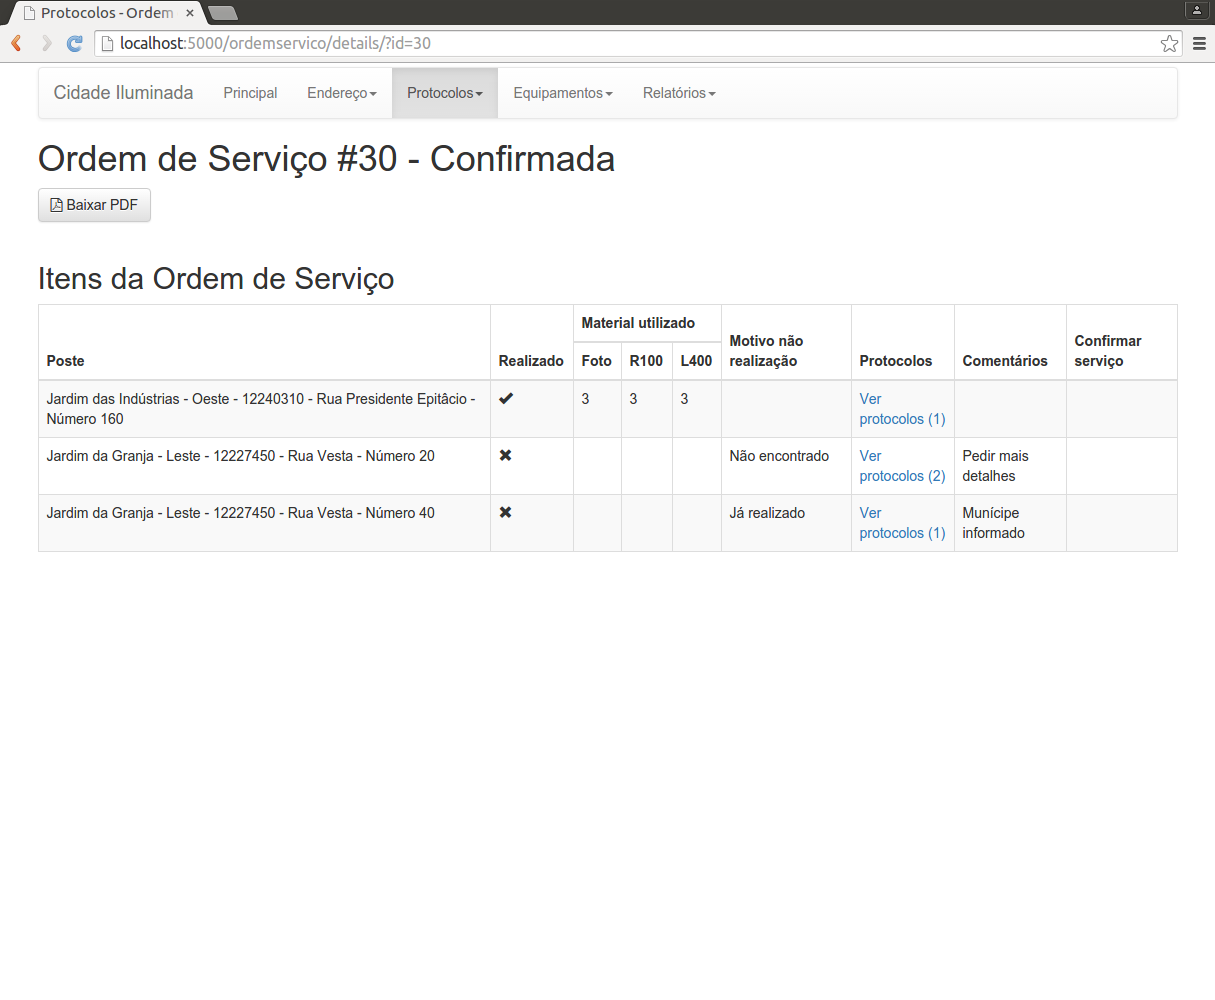
\includegraphics[scale=0.25]{site/20-os_confirmada.png}
 \legend{Fonte: Produzido pelos autores}
\end{figure}

\clearpage

% ---
% Finaliza a parte no bookmark do PDF, para que se inicie o bookmark na raiz
% ---
\bookmarksetup{startatroot}%
% ---

% ---
% Conclusão
% ---
\section*{Conclusão}
\addcontentsline{toc}{section}{Conclusão}

A gestão de pendencias relativas a iluminação pública da prefeitura de São José dos Campos é burocrática, o que reflete na lentidão do atendimento e manutenção de um serviço tão essencial ao bem estar e segurança da população.
O fato da responsabilidade pela manutenção ter sido passada para as prefeituras recentemente também é um fator crítico no desempenho do atendimento, já que as prefeituras tiveram que se adaptar rapidamente.

Partindo desta problemática, incentivados pela ideia de agilizar este processo, desenvolvemos o projeto Cidade Iluminada, onde o ambiente web, que passou pela validação da equipe da Secretaria de Obras da Prefeitura Municipal de São José dos Campos provou reduzir a carga de trabalho e facilitar o recolhimento e análise das denuncias recebidas, automatizando um trabalho que era feito manualmente.

Infelizmente o aplicativo ainda não será disponibilizado para os munícipes a pedido do cliente, que alega que este novo canal de comunicação poderia neste primeiro momento congestionar os recebimentos de chamadas já existente, tendo em vista que a equipe ainda não possui um processo estruturado para a demanda.
Em primeiro momento, o aplicativo será usado pelos próprios funcionários da Secretaria de Obras para a identificação de pontos de iluminação defeituosos.

\subsection{Trabalhos futuros e melhorias}

Como trabalho futuro, foi proposto que o aplicativo seja liberado para o uso dos munícipes, integrando ao ambiente web para que ele receba as denúncias diretamente.
Para que o aplicativo seja liberado, também é necessário que além de Android seja desenvolvido para iOS assim alcançando todos os públicos.

Como melhorias, seria interessante que futuramente novas funcionalidades sejam integradas, utilizando o aplicativo para outros tipos de chamadas relacionadas ou não com a iluminação pública, como por exemplo, abrir chamados para o conserto de buracos de rua, árvores caídas, etc..

Além disso, é possível fazer grandes melhorias da interface gráfica dos aplicativos, tornando o ambiente web mais amigável para o uso de funcionários com vários níveis de conhecimento em informática.

% ----------------------------------------------------------
% ELEMENTOS PÓS-TEXTUAIS
% ----------------------------------------------------------
\postextual

% ---
% Título e resumo em língua estrangeira
% ---

% \twocolumn[    		% INICIO DE ARTIGO EM DUAS COLUNAS

% titulo em inglês
\titulo{Public lighting maintenance management system \\ CidadeIluminada}
\emptythanks
\maketitle
\renewcommand{\resumoname}{Abstract}
\begin{resumoumacoluna}
 \begin{otherlanguage*}{english}
   This paper presents a study on mobile development, explaining the
   implementation of a software prototype that will assist in receiving
   complaints and analysis related to street lighting in the city of São José
   dos Campos. The application was developed on Android and will be responsible
   for sending these complaints to a web environment. The web application
   will be responsible for responding to requests from the Android application
   and process them so that the maintenance of public lighting points is done
   in a faster and less bureaucratic way.
   \vspace{\onelineskip}

   \noindent
   \textbf{Keywords}: Public lighting system. Android Application. Web system for maintenance.
 \end{otherlanguage*}
\end{resumoumacoluna}

% ]  				% FIM DE ARTIGO EM DUAS COLUNAS
% ---

% ----------------------------------------------------------
% Referências bibliográficas
% ----------------------------------------------------------
\bibliography{bibliografia}

\end{document}
